% Chapter Template

\chapter{Estado del Arte} % Main chapter title

% \label{Chapter2} 

% La revisión del estado del arte tiene varias facetas. Por un lado, se encuentra el estado del arte relacionado a los fenómenos físicos que implican el estudio de los índicies de vegetación a partir de imágenes de cámaras multiespectrales. Así se pueden definir tópicos relacionados al tema de investigación. Estos tópicos, para este trabajo, se definen de la siguiente forma:

% \begin{itemize}
%     \item Índices de vegetación
%     \item Óptica
%     \item Sensores ópticos
%     \item Procesamiento de imágenes
% \end{itemize}


% \begin{figure}[htbp]
%     \centering
%     \includesvg[width=0.8\textwidth, inkscapelatex=false]{Figures/estado_del_arte} % Cambia 'imagen.svg' al nombre de tu archivo SVG
%     \caption{Estructura del estado del arte}
%     \label{fig:estado del arte}
% \end{figure}

% \subsection{Palabras claves}

% Para crear la ecuación de búsqueda bibliográfica, se utilizan las siguientes palabras claves:

% \begin{table}[htbp]
% \centering
% \caption{Resumen de Ecuaciones de Búsqueda Bibliográfica}
% \label{tab:resumen_ecuaciones}
% \begin{tabular}{|c|c|}
% \hline
% \textbf{Área} & \textbf{Palabras Clave} \\ \hline
% \multirow{6}{*}{Óptica} & Digital Image Processing \\
%  & Remote sensing \\
%  & Aberrations \\
%  & Camera \\
%  & NIR \\
%  & Visible \\ \hline
% \multirow{4}{*}{Métodos matemáticos} & Remote sensing \\
%  & Statistics \\
%  & Image processing \\
%  & Camera AND Satellite \\ \hline
% \multirow{3}{*}{Índices de vegetación} & Vegetation indices \\
%  & Remote sensing \\ \hline
% \end{tabular}
% \end{table}

% \end{itemize}




% \section{Principios ópticos y electromagnéticos}


% Este segmento del estado del arte aborda los fundamentos teóricos de las ondas electromagnéticas y las ecuaciones de Fresnel, que son esenciales para comprender los mecanismos de interacción de la luz con diferentes medios en el contexto de la teledetección y la óptica.\\

% Las ecuaciones de Maxwell constituyen la base para describir el comportamiento de los campos eléctricos y magnéticos, así como su interacción con la materia. En el contexto de la óptica y el sensado remoto, estas ecuaciones son fundamentales para entender cómo las ondas electromagnéticas se propagan a través de diferentes medios, sean isotrópicos o anisotrópicos.


% Las ecuaciones de Maxwell describen cómo los campos eléctricos y magnéticos se generan y modifican mutuamente, así como por cargas y corrientes. Estas ecuaciones son:

% \begin{equation}
%     \nabla \cdot \mathbf{E} = \frac{\rho}{\epsilon_0}
% \end{equation}

% \begin{equation}
%     \nabla \cdot \mathbf{B} = 0
% \end{equation}

% \begin{equation}
%     \nabla \times \mathbf{E} = -\frac{\partial \mathbf{B}}{\partial t}
% \end{equation}

% \begin{equation}
%     \nabla \times \mathbf{B} = \mu_0 \mathbf{J} + \mu_0 \epsilon_0 \frac{\partial \mathbf{E}}{\partial t}
% \end{equation}
% donde \(\mathbf{E}\) y \(\mathbf{B}\) son los campos eléctrico y magnético, \(\rho\) es la densidad de carga, \(\mathbf{J}\) es la densidad de corriente, \(\epsilon_0\) es la permitividad del vacío, y \(\mu_0\) es la permeabilidad del vacío.


% En medios isotrópicos, las propiedades del medio son uniformes en todas las direcciones. Esto simplifica la solución de las ecuaciones de Maxwell, ya que los parámetros del medio no dependen de la dirección de propagación de la onda. Las ondas electromagnéticas en estos medios se caracterizan por su velocidad de propagación \( c = \frac{1}{\sqrt{\epsilon \mu}} \), donde \(\epsilon\) y \(\mu\) son la permitividad y la permeabilidad del medio, respectivamente.


% Los medios anisotrópicos, como ciertos cristales y materiales birrefringentes, poseen propiedades ópticas que varían según la dirección. En estos medios, las ecuaciones de Maxwell deben modificarse para reflejar la anisotropía mediante tensores de permitividad y permeabilidad, lo que resulta en una descripción más compleja de la propagación de las ondas. Las soluciones típicas en estos medios no son ondas planas simples, sino modos que dependen de la orientación del cristal \cite{ImagingOptics}.


% En la teledetección, la comprensión de la propagación de ondas en medios anisotrópicos es crucial para el diseño de sistemas que puedan discriminar entre diferentes tipos de superficies y orientaciones. Esto es especialmente importante en la teledetección polarimétrica, donde la anisotropía del medio puede afectar significativamente la polarización de las ondas reflejadas o transmitidas \cite{Bravo-Aranda2016PBLPOLARIS}.


% Las ondas electromagnéticas son perturbaciones en los campos eléctricos y magnéticos que se propagan a través del espacio sin necesidad de un medio físico. Estas ondas se caracterizan por su longitud de onda (\(\lambda\)) y frecuencia (\(f\)), relacionadas por la velocidad de la luz (\(c\)), donde \(c = \lambda f\). Estas ondas pueden ser descritas por las ecuaciones de Maxwell, que formulan cómo los campos eléctricos (\(\mathbf{E}\)) y magnéticos (\(\mathbf{B}\)) se generan y alteran uno al otro así como a las cargas y corrientes eléctricas \cite{Volosyuk2018PhenomenologicalSystems}.


% Cuando las ondas electromagnéticas encuentran un cambio en el medio a través del cual se propagan, parte de la energía se refleja y otra parte se transmite a través del nuevo medio. Las ecuaciones de Fresnel describen cuantitativamente estas interacciones en la interfaz entre dos medios con índices de refracción diferentes. Estas ecuaciones son cruciales para calcular la reflectancia y transmitancia, proporcionando los coeficientes de reflexión (\(r\)) y transmisión (\(t\)) que dependen del ángulo de incidencia y las propiedades del material:

% \begin{equation}
%     r_{\parallel} = \frac{n_2 \cos \theta_i - n_1 \cos \theta_t}{n_2 \cos \theta_i + n_1 \cos \theta_t}
% \end{equation}

% \begin{equation}
%     t_{\parallel} = \frac{2 n_1 \cos \theta_i}{n_2 \cos \theta_i + n_1 \cos \theta_t}
% \end{equation}

% \begin{equation}
%     r_{\perp} = \frac{n_1 \cos \theta_i - n_2 \cos \theta_t}{n_1 \cos \theta_i + n_2 \cos \theta_t}
% \end{equation}

% \begin{equation}
%     t_{\perp} = \frac{2 n_1 \cos \theta_i}{n_1 \cos \theta_i + n_2 \cos \theta_t}
% \end{equation}


% Estos coeficientes diferencian entre los modos de polarización paralela (\(\parallel\)) y perpendicular (\(\perp\)) de la onda incidente \cite{Jin1994ElectromagneticSensing}.


% Las ecuaciones de Fresnel son fundamentales para diseñar instrumentos ópticos y sensores de teledetección, permitiendo a los científicos modelar y predecir cómo las señales electromagnéticas interactúan con la atmósfera y la superficie terrestre. Estos modelos son esenciales para interpretar correctamente los datos recogidos por satélites y otros sensores remotos, optimizando así la recolección de datos sobre la composición química, estructura física y variaciones temporales de los cuerpos observados \cite{Hartl1989FUNDAMENTALSSENSING}.




% El espectro electromagnético abarca todas las formas de radiación electromagnética, cada una caracterizada por su longitud de onda o frecuencia. Estas radiaciones varían desde las ondas de radio de gran longitud de onda hasta los rayos gamma de corta longitud de onda, pasando por el espectro visible que percibe el ojo humano.


% El espectro electromagnético se compone de radiación de radio, microondas, infrarrojo, luz visible, ultravioleta, rayos X y rayos gamma. Esta diversidad de bandas se utiliza de manera extensiva en teledetección para obtener información detallada de la Tierra y otros cuerpos celestes desde el espacio.





% \begin{figure}[htbp]
%     \centering
%     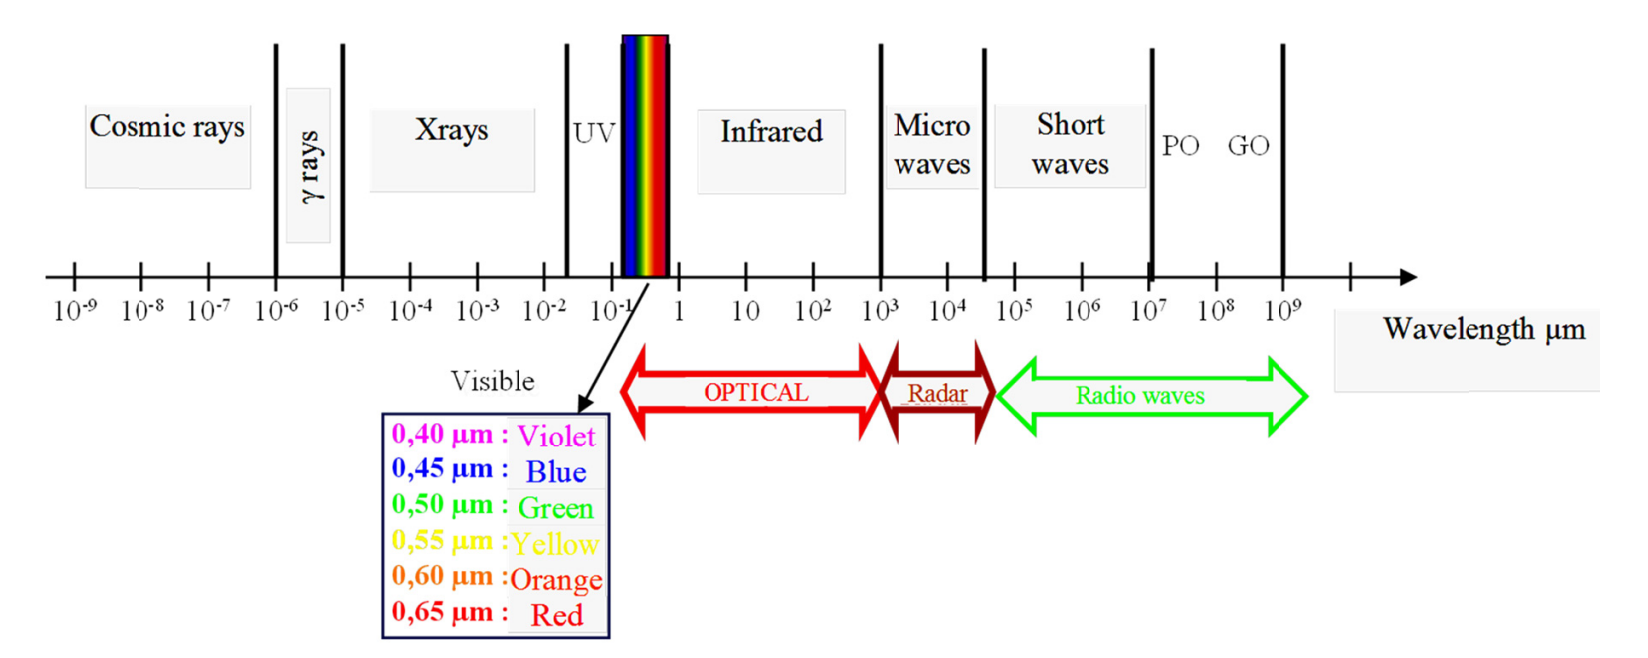
\includegraphics[width=\textwidth]{Figures/C2/espectro.png} % Cambia 'imagen.svg' al nombre de tu archivo SVG
%     \caption{Espectro electromagnético (falta formatear y referenciar). Tomado de \cite{BaghdadiOpticalMethods}.}
%     \label{fig:imagen}
% \end{figure}

% \section{Interacción radiación-materia}

% Esta sección esta destinada a describir físicamente las definiciones y conceptos esenciales para comprende la señal medida con un instrumento óptico. El área de la ciencia que mide la radiación es llamada radiometría. La transferencia radiativa describe interacción radiación-materia. La radiación puede ser modelada como una onda que se propaga por el espacio con determinadas características como: su longitud de onda, su velocidad de propagación, su intensidad, su fase y su estado de polarización.

% En teledetección, cada rango del espectro tiene aplicaciones específicas basadas en su interacción con la atmósfera y la superficie terrestre. Por ejemplo, las ondas de radio son útiles para penetrar nubes y capturar imágenes independientemente de la luz solar, mientras que las imágenes en el espectro visible proporcionan una representación cercana a lo que percibe el ojo humano.


% La radiación en diferentes partes del espectro electromagnético tiene propiedades únicas. Las radiaciones más energéticas, como los rayos X y los rayos gamma, tienen longitudes de onda cortas y alta frecuencia, lo que les permite penetrar a través de materiales sólidos, una propiedad utilizada en aplicaciones médicas y de seguridad. En contraste, las ondas de radio tienen longitudes de onda más largas y frecuencias más bajas, adecuadas para la comunicación a larga distancia.



% \subsection{Propiedades radiativas de la materia}

% \subsubsection{Noción de reflectancia}
% La reflectancia se define como la proporción de la radiación electromagnética que es reflejada por una superficie en comparación con la que incide sobre ella. Este coeficiente es crucial para entender cómo diversas superficies absorben y reflejan la energía solar en distintas longitudes de onda del espectro electromagnético.

% Cuando la radiación incide en una superficie, parte de esta energía es reflejada, otra absorbida, y una fracción transmitida. La cantidad reflejada depende de las propiedades del material y de la longitud de onda de la radiación incidente. Matemáticamente, la reflectancia (\(R\)) se expresa como:

% \begin{equation}
%     R(\lambda) = \frac{I_r(\lambda)}{I_i(\lambda)}
% \end{equation}

% donde \(I_r(\lambda)\) es la intensidad de la radiación reflejada e \(I_i(\lambda)\) es la intensidad de la radiación incidente, ambas en la longitud de onda \(\lambda\).

% La reflectancia de una superficie puede variar con la dirección e incluye dependencias de la geometría de iluminación y observación. En teledetección, se usa el concepto de reflectancia bidireccional para analizar cómo varía la reflectancia con los ángulos de iluminación y observación.

% Además, la reflectancia es fundamental para modelar el albedo de la Tierra, esencial en estudios sobre el balance energético y el cambio climático.

% En teledetección, se utiliza para caracterizar y clasificar diferentes tipos de coberturas terrestres mediante sus firmas espectrales. Por ejemplo, la vegetación sana muestra mayor reflectancia en el infrarrojo cercano y menor en el rojo visible, lo que es la base para índices de vegetación como el NDVI.

% La calibración radiométrica de los sensores y la corrección de los efectos atmosféricos son esenciales para obtener mediciones precisas de reflectancia, lo que permite comparar datos a lo largo del tiempo y del espacio.

% \begin{figure}[htbp]
%     \centering
%     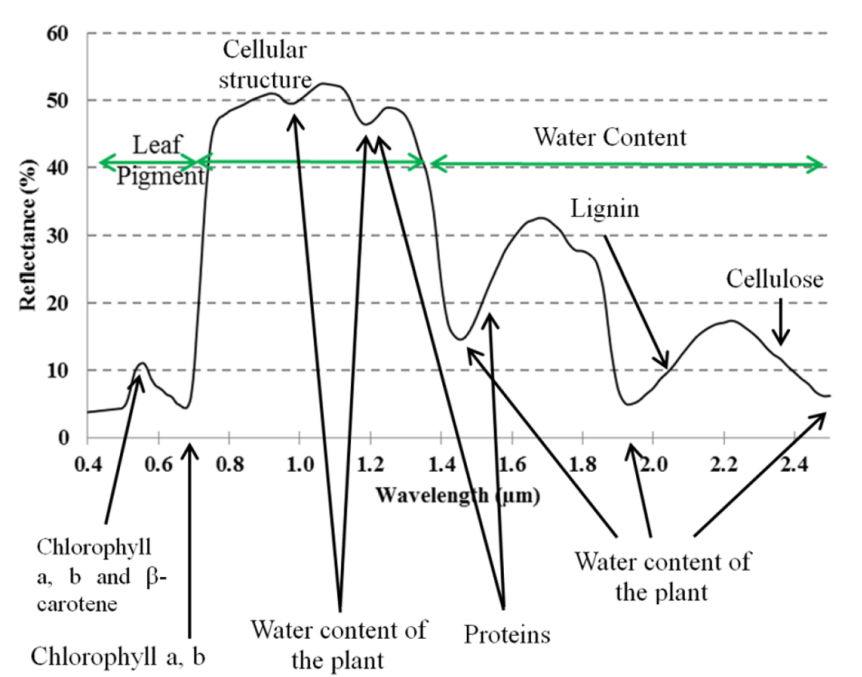
\includegraphics[width=0.7\textwidth]{Figures/C2/reflectancia.png}
%     \caption{Reflectancia de múltiples objetos. Tomado de \cite{BaghdadiOpticalMethods}.}
%     \label{fig:refl}
% \end{figure}

% \subsubsection{Noción de absorbancia}

% La absorbancia mide la cantidad de luz que una muestra absorbe al pasar a través de ella. Se define como el logaritmo negativo de la transmitancia (\(T\)):

% \begin{equation}
%     A = -\log_{10}(T) = -\log_{10}\left(\frac{I}{I_0}\right)
% \end{equation}

% donde \(I\) es la intensidad de la luz transmitida y \(I_0\) la intensidad de la luz incidente. La relación entre el coeficiente de absorción (\(\alpha\)) y la absorbancia en un medio homogéneo se describe mediante la ley de Beer-Lambert:

% \begin{equation}
%     A = \alpha \cdot l \cdot c
% \end{equation}

% donde \(l\) es la longitud del camino óptico y \(c\) la concentración del absorbente. Esta propiedad es vital para el análisis en teledetección y otras aplicaciones, desde el monitoreo de la calidad del agua hasta la evaluación de la salud vegetal.

% \subsubsection{Noción de transmitancia}
% La transmitancia indica la proporción de luz que atraviesa una sustancia respecto a la luz incidente, definida como:

% \begin{equation}
%     T = \frac{I}{I_0}
% \end{equation}

% Está inversamente relacionada con la absorbancia, y su estudio es crucial en teledetección para modelar y corregir los efectos atmosféricos en imágenes de satélite, mejorando la precisión de las observaciones de la superficie terrestre.

% \subsubsection{Noción de difusión}


% \section{Imagen (Cambiar por procesamiento de imagenes)}



% \begin{enumerate}
%     \item 
% \end{enumerate}

% \subsection{Concepto de imágen}
% \subsection{Sistemas fromadores de imágenes}



% \begin{figure}[htbp]
%     \centering
%     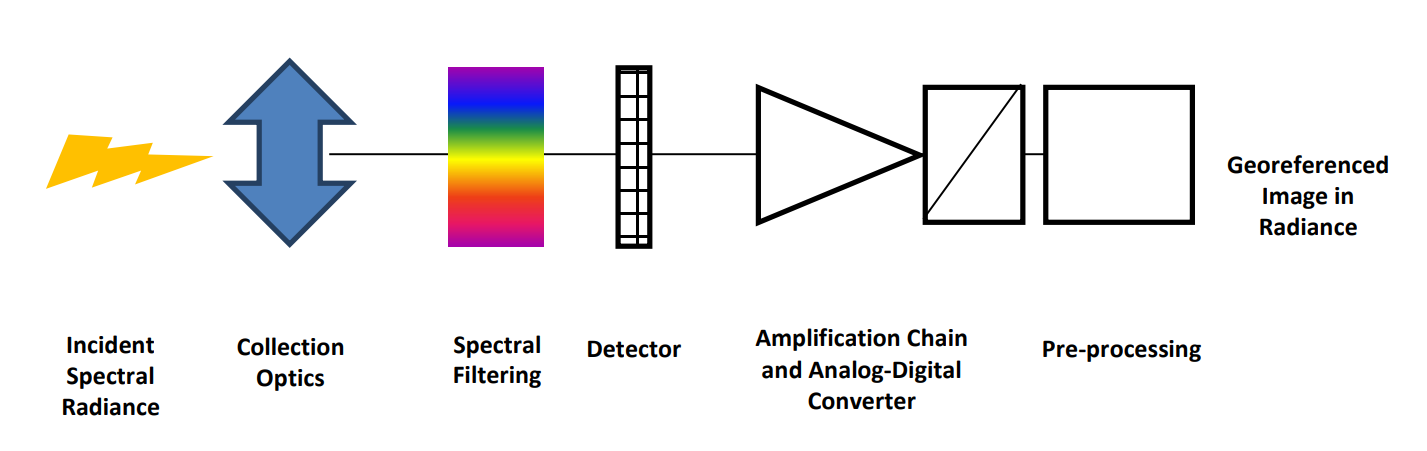
\includegraphics[width=0.9\textwidth]{Figures/C2/esquea_sis_imagen.png}
%     \caption{Esquema de un sistema formador de imagen. Tomado de \cite{BaghdadiOpticalMethods}.}
%     \label{fig:esq_sis_ima}
% \end{figure}

% \subsection{Sensores ópticos}


% %% Al-Hourani2023LinePlatforms
% El uso de cámaras multiespectrales montadas en plataformas UAV (vehículos aéreos no tripulados) se ha vuelto cada vez más común en el monitoreo agrícola y ambiental. Estas tecnologías permiten la evaluación precisa de la vegetación mediante la captura de información espectral detallada que puede ser utilizada para calcular índices de vegetación como el NDVI (Índice de Vegetación de Diferencia Normalizada). Este estado del arte revisa los principios de operación y el diseño de cámaras multiespectrales, con un enfoque en el artículo “Line Scan Hyperspectral Imaging Framework for Open Applications”.

% \subsubsection{Principios Matemáticos del Sistema de Imágenes Hiperespectrales}
% El sistema de imágenes hiperespectrales propuesto en el artículo utiliza un enfoque de escaneo en línea (line-scan), también conocido como escaneo de empuje (push broom), donde la escena se escanea línea por línea. La imagen hiperespectral resultante es un cubo de datos 3D $H(x, y, \lambda)$, con dos dimensiones representando características espaciales ($x$, $y$) y la tercera dimensión representando la información espectral $\lambda$ \cite{line_scan_hyperspectral}.

% Matemáticamente, cada línea escaneada es dispersada espectralmente usando un sistema de lentes y un espectroscopio, proyectando un espectro sobre un sensor CMOS. La intensidad de la imagen monocromática para un píxel en particular se calcula mediante:

% \[
% \tilde{I}_{\text{mono}}(x, y) = f \left( A \cdot T \cdot \int_{\lambda_{\text{min}}}^{\lambda_{\text{max}}} g(\lambda) \cdot s(\lambda) \, d\lambda \right)
% \]

% donde $A$ es el área del sensor, $T$ es el tiempo de exposición, $g(\lambda)$ es la irradiancia espectral, y $s(\lambda)$ es la sensibilidad espectral del sensor \cite{line_scan_hyperspectral}.

% \subsubsection{Diseño del Sistema de Cámaras Multiespectrales}
% El diseño del sistema multiespectral descrito en el artículo se enfoca en utilizar componentes accesibles y de bajo costo para construir una plataforma asequible. La plataforma incluye un sistema optomecánico que emplea espejos de galvanómetro para escanear la escena en un eje, mientras que una lente de montaje CS y un espectroscopio sencillo permiten la captura de imágenes espectrales \cite{Al-Hourani2023LinePlatforms}.

% El sistema diseñado fue evaluado comparando los resultados espectrales con mediciones realizadas por espectrómetros comerciales de gama alta, mostrando una precisión espectral comparable a pesar del bajo costo de los componentes utilizados. La metodología de escaneo en línea permitió capturar datos espectrales con alta resolución espacial y espectral, cruciales para la determinación precisa de índices de vegetación \cite{Al-Hourani2023LinePlatforms}.

% La integración de cámaras multiespectrales en UAVs para el monitoreo de la vegetación es una herramienta poderosa para la agricultura de precisión. Los desarrollos presentados en el artículo demuestran que es posible construir sistemas eficientes y de bajo costo que puedan capturar información espectral detallada, lo que facilita la evaluación precisa de la salud de los cultivos mediante la determinación de índices de vegetación.

% Estos avances en la tecnología de imágenes hiperespectrales y su aplicación en UAVs prometen mejorar significativamente las prácticas agrícolas y el monitoreo ambiental, proporcionando datos críticos para la toma de decisiones informada.

% \subsection{Óptica de Imágenes para sistemas hiperespectrales (HSI)}

% En la teledetección y, particularmente, en el estudio de índices de vegetación, la imagen hiperespectral (HSI) es una herramienta poderosa para capturar información detallada sobre la composición espectral de la vegetación y otros objetos en la Tierra. La imagen HSI se representa como un cubo de datos tridimensional que incluye dos dimensiones espaciales y una tercera dimensión que captura la información espectral. Este cubo se conoce como "cubo hiperespectral" \cite{Al-Hourani2023LinePlatforms}.

% Existen varios métodos para adquirir este cubo de datos 3D:

% \begin{enumerate}
%     \item \textbf{Escaneo puntual (whiskbroom)}: Este método escanea individualmente cada punto de la escena y obtiene la información espectral para cada píxel [x, y]. Aunque proporciona una alta resolución espectral, su proceso es lento debido a la necesidad de capturar punto por punto.

%     \item \textbf{Escaneo de banda espectral (framing)}: En este método, la imagen proyectada pasa a través de filtros de banda pasante sintonizables, que permiten solo una parte estrecha del espectro a la vez. Luego, el filtro se desplaza a través del espectro. A pesar de ser más rápido que el método whiskbroom, requiere filtros costosos que ofrezcan velocidad y precisión.

%     \item \textbf{Método de instantánea (snapshot)}: Aquí, la escena se duplica ópticamente en múltiples réplicas pequeñas, y cada réplica pasa por un filtro de banda estrecha. Este método permite una adquisición más rápida y es conocido como "método de instantánea". Sin embargo, requiere sistemas ópticos microfabricados especializados, lo cual puede ser costoso y técnicamente complejo.

%     \item \textbf{Escaneo lineal (push broom)}: Este método, adoptado en muchas aplicaciones de HSI debido a su eficiencia, escanea la escena línea por línea. Cada línea escaneada se extiende en una imagen espatio-espectral 2D [y, z], y estas imágenes se apilan para formar el cubo de datos hiperespectrales [x, y, z]. 
% \end{enumerate}

% En este método, se emplea un espectrógrafo típico que dispersa la luz de la línea escaneada, convirtiéndola en una imagen espatio-espectral 2D. El proceso implica usar una lente de imagen que forma una imagen real del objetivo en una rendija estrecha, seguida de lentes colimadoras para dirigir la luz colimada hacia ópticas dispersivas, como un prisma óptico o una red de difracción.

% \begin{itemize}
%     \item \textbf{Prismas ópticos}: Ofrecen bajas pérdidas de transmisión pero presentan una dispersión espectral no lineal, lo que requiere una cuidadosa calibración.

%     \item \textbf{Redes de difracción}: Dispersan la luz de manera lineal, lo que simplifica la calibración. La configuración típica es un sistema prismático donde la red de difracción se encuentra entre dos prismas, asegurando que la entrada y salida de la luz estén alineadas.
% \end{itemize}

% \subsection{Aplicación de Sensores}

% Una vez dispersada la luz en sus componentes espectrales, un sensor óptico, como un sensor CMOS (Complementary Metal-Oxide-Semiconductor), captura la imagen espatio-espectral. Aunque los sensores CMOS tienen ciertas limitaciones en términos de ruido y rango de longitud de onda (particularmente en el infrarrojo cercano), su velocidad de lectura y bajo costo los hacen adecuados para muchas aplicaciones de teledetección. En casos donde se requieren rangos de longitud de onda más allá del infrarrojo cercano, materiales especializados como el telururo de cadmio de mercurio (MCT) pueden ser utilizados, aunque a un costo más elevado.

% \subsection{Relevancia para la Teledetección y los Índices de Vegetación}

% La capacidad de capturar información espectral detallada permite que los sistemas de imágenes hiperespectrales sean utilizados para calcular índices de vegetación con precisión, proporcionando datos cruciales para la evaluación de la salud de las plantas, el monitoreo del estrés hídrico, y la gestión de recursos agrícolas. Estos métodos ópticos y el uso de sensores avanzados en la adquisición de imágenes multiespectrales son fundamentales para aplicaciones precisas de agricultura y monitoreo ambiental.



% \section{Índices de vegetación}

% En la investigación ambiental, los cocientes de bandas son frecuentemente utilizados como índices de vegetación con el fin de cuantificar la cantidad de vegetación que puede aparecer en una imagen digital multiespectral \cite{Vaiopoulos2004TheIndices}. La relación matemática general de un índice de vegetación, $R$, formado por el cociente de bandas, puede escribirse como:

% \begin{equation}
% R = \frac{a_1x + a_2y + a_3}{b_1x + b_2y + b_3}
% \end{equation}

% donde $x$ e $y$ son los valores de brillo de los píxeles (o valores de reflectancia) en la banda del infrarrojo cercano (NIR) y la banda roja, respectivamente. Los coeficientes $a_1, a_2, a_3, b_1, b_2$ y $b_3$ son definidos usualmente por criterios empíricos para mejorar la sensibilidad del índice de vegetación a diferentes tipos de cobertura terrestre \cite{Vaiopoulos2004TheIndices}.

% En algunos casos, en lugar de $R$, se utiliza una función de $R$ (como la raíz cuadrada de $R$ o $R$ multiplicado por una constante) para definir el índice de vegetación.

% \begin{equation}
% \text{SVI} = \frac{x}{y}
% \end{equation}

% Este índice de vegetación conocido como Simple Ratio Index (SVI) utiliza el cociente entre las reflectancias en el infrarrojo cercano y el rojo, proporcionando una medida simple de la cantidad de vegetación en la escena \cite{Vaiopoulos2004TheIndices}.


% %% Myneni1995TheIndexes

% El uso de índices espectrales de vegetación en la teledetección ha permitido importantes avances en la monitorización y cuantificación de la vegetación a nivel global. Myneni et al. (1995) en su artículo \textit{The Interpretation of Spectral Vegetation Indexes} \cite{Myneni1995TheIndexes}, destacan que los índices espectrales de vegetación pueden correlacionarse con parámetros clave como el área foliar, la biomasa y el funcionamiento fisiológico de la vegetación.

% Los índices de vegetación se clasifican en tres tipos principales:


% \subsection{Tipo I: Índices Lineales}
% Un ejemplo común de índices lineales es el Índice de Vegetación de Diferencia Normalizada (NDVI), que mide el contraste entre la reflectancia en el rojo (absorción por la clorofila) y el infrarrojo cercano (reflejado por la estructura celular de las hojas).

% \begin{equation}
%     \text{NDVI} = \frac{(NIR - Red)}{(NIR + Red)}
% \end{equation}

% Donde:
% \begin{itemize}
%     \item $NIR$: Reflectancia en el infrarrojo cercano (0.75-1.35 µm).
%     \item $Red$: Reflectancia en la banda del rojo (0.6-0.7 µm).
% \end{itemize}

% \subsection{Tipo II: Índices No Lineales}
% Este tipo de índices utiliza productos de reflectancia para minimizar efectos atmosféricos. Un ejemplo es el Índice de Monitoreo del Medio Ambiente Global (GEMI), que se expresa de la siguiente manera:

% \begin{equation}
%     \eta = \frac{2 \cdot (NIR^2 - Red^2)}{NIR + Red + 0.5}
% \end{equation}

% \begin{equation}
%     \text{GEMI} = \eta \cdot (1 - 0.25 \cdot \eta) - \frac{(Red - 0.125)}{1 - Red}
% \end{equation}

% \subsection{Tipo III: Índices Derivados de Segunda Orden}
% Estos índices corrigen los efectos atmosféricos y del suelo. El Índice de Vegetación Atmosféricamente Resistente (ARVI) usa bandas adicionales como la del azul para realizar estas correcciones:

% \begin{equation}
%     \text{ARVI} = \frac{(NIR - (2 \cdot Red - Blue))}{(NIR + (2 \cdot Red + Blue))}
% \end{equation}

% Donde:
% \begin{itemize}
%     \item $Blue$: Reflectancia en la banda del azul (alrededor de 0.45 µm).
% \end{itemize}

% Los autores \cite{Myneni1995TheIndexes} concluyen que los índices espectrales de vegetación son indicadores fiables de la abundancia de clorofila y la absorción de energía por la vegetación. Esto permite su aplicación en estudios a gran escala, como el monitoreo del crecimiento de cultivos y la evaluación de la fracción de radiación fotosintéticamente activa absorbida. Además, estos índices se saturan en altas concentraciones de biomasa, lo que puede limitar su aplicabilidad en ecosistemas muy densos.

% Este trabajo establece una base teórica sólida para la teledetección espectral de la vegetación, al correlacionar las características ópticas de la vegetación con los índices derivados de la reflectancia espectral, facilitando así aplicaciones en estudios globales de la biosfera terrestre.

% \section{Teledetección de índices de vegetación mediante imágenes}



% %% Bazrafkan et al. (2023)
% Bazrafkan et al. (2023) evaluaron cinco algoritmos de aprendizaje automático para predecir la madurez de los guisantes secos en parcelas de campo, utilizando datos recopilados por UAS. Los algoritmos consideraron una variedad de variables, incluyendo métricas de altura de cultivos, bandas espectrales estrechas y 18 índices de vegetación de color y espectrales distintos. La eliminación hacia atrás de características se utilizó para optimizar el rendimiento predictivo del modelo \cite{Bazrafkan2023PredictingUASs}.
% El estudio reveló que el enfoque más efectivo para evaluar la madurez de los guisantes secos involucraba una combinación de bandas espectrales estrechas, borde rojo, NIR, y índices de vegetación basados en RGB, junto con métricas de textura de imágenes y métricas de altura de cultivos. La implementación de un modelo de bosque aleatorio mejoró aún más la precisión de los resultados, mostrando el mayor nivel de precisión con un valor de 0.99 para las tres métricas de precisión, recall y puntajes f1 \cite{Bazrafkan2023PredictingUASs}.

% %% Deng et al. (2018)
% La metodología aplicada por Deng et al. (2018) incluyó un flujo de trabajo detallado para el procesamiento de imágenes de Mini-MCA6, que comprendió la corrección de ruido, corrección de viñeteo, alineación de banda a banda, y calibración radiométrica utilizando métodos como el lineal empírico (EL) y la línea empírica de subbanda (SEL). Este enfoque meticuloso permitió generar ortomosaicos georreferenciados de seis bandas con alta precisión \cite{Deng2018UAV-basedCameras}.
% Deng et al. (2018) observaron que la precisión de los valores de reflectancia de la cámara Mini-MCA6 era superior a la de la cámara Sequoia, particularmente cuando se utilizaba el método de calibración adecuado. En términos de predicción de valores SPAD, el reNDVI mostró un mejor desempeño que el NDVI en todas las condiciones de tratamiento de nitrógeno, independientemente de la cámara utilizada. Este hallazgo subraya la relevancia del reNDVI para evaluar el estado nutricional de los cultivos, especialmente en condiciones de campo variadas \cite{Deng2018UAV-basedCameras}.


% %% Vuletić et al
% El estudio realizado por Vuletić et al. se centra en la imagen multiespectral de corto alcance utilizando un sistema MS-D. Este sistema emplea cámaras multiespectrales calibradas con respecto a una cámara RGB-D para la inscripción precisa de imágenes, esencial para el monitoreo y la evaluación de la salud de los cultivos mediante índices de vegetación \cite{Vuletic2023Close-rangeSystem}. El sistema MS-D demostró superioridad sobre los métodos basados en características tradicionales en diversas pruebas, incluyendo la inscripción de imágenes en entornos reales y simulados. Esto se traduce en una mayor precisión para la evaluación del estrés hídrico en plantas, mostrando cambios significativos en índices como NDVI y NDRE en condiciones controladas de estrés por riego \cite{Vuletic2023Close-rangeSystem}. El sistema MS-D se presenta como una herramienta robusta, rápida y precisa, adecuada para el monitoreo de plantas sin la necesidad de recalibración entre usos, facilitando su aplicación en entornos agrícolas variados \cite{Vuletic2023Close-rangeSystem}.

% % Smeesters2023Wide-Field-of-ViewMonitoring
% El diseño de cámaras multiespectrales de amplio campo de visión para la monitorización continua del césped se aborda mediante un sistema de cinco canales que cubre las bandas del visible, infrarrojo cercano y térmico. Se optimiza el diseño de la cámara para un amplio campo de visión, permitiendo la integración en dispositivos de iluminación y la evaluación autónoma y continua del estrés hídrico y la presencia de enfermedades o plagas en las plantas \cite{Smeesters2023Wide-Field-of-ViewMonitoring}. Los resultados demuestran una calidad de imagen excepcional en todos los canales de imagen, confirmada por una función de transferencia de modulación (MTF) que supera un contraste de 0.5 en una frecuencia espacial de 72 líneas por milímetro para los diseños de imagen visible e infrarroja cercana. Este sistema propuesto supera las limitaciones de los sistemas tradicionales montados en UAVs, que suelen tener un campo de visión reducido \cite{Smeesters2023Wide-Field-of-ViewMonitoring}. El estudio concluye que el diseño de la cámara multispectral de campo visual amplio es viable para el monitoreo automatizado y continuo de campos de césped, optimizando el uso de recursos y minimizando la necesidad de intervenciones manuales frecuentes. Esta tecnología podría adaptarse para una variedad de aplicaciones agrícolas donde el monitoreo continuo es crucial \cite{Smeesters2023Wide-Field-of-ViewMonitoring}.

% % Silva et al.
% Silva et al. \cite{Orlando2023POTENTIALIRRIGATION} investigan la monitorización de la irrigación de cultivos de café utilizando imágenes multiespectrales obtenidas por sensores incorporados en vehículos aéreos no tripulados (UAV). El estudio evalúa la capacidad de cámaras de bajo costo para discriminar diferentes tratamientos de agua en el cultivo de café, utilizando el Potencial Hídrico Foliar (LWP) como indicador. La metodología consiste en la captura de imágenes multiespectrales a través de un UAV equipado con una cámara Mapir Survey3W. La cámara capta bandas del espectro visible, NIR y red. La evaluación del LWP se realiza in situ, utilizando una cámara de presión de Scholander para medir el potencial hídrico de las hojas del café durante diferentes etapas del ciclo de irrigación. Se emplean técnicas de aprendizaje automático para modelar y predecir el LWP a partir de los índices de vegetación derivados de las imágenes \cite{Orlando2023POTENTIALIRRIGATION}. Los resultados demuestran que el índice de vegetación NDVI, derivado de las imágenes multiespectrales, permite una discriminación efectiva de los diferentes regímenes de riego aplicados. El modelo de árbol aleatorio y el algoritmo SMOreg destacan por su capacidad para predecir el LWP con un bajo error cuadrático medio (RMSE), lo que indica un alto grado de precisión en la detección del estrés hídrico en el cultivo de café \cite{Orlando2023POTENTIALIRRIGATION}. El estudio concluye que las imágenes multiespectrales capturadas por UAVs, combinadas con técnicas avanzadas de procesamiento de datos y aprendizaje automático, ofrecen una metodología prometedora para la monitorización precisa y en tiempo real de la irrigación en cultivos de café. Esta tecnología tiene el potencial de mejorar la gestión del agua en la agricultura, optimizando el uso de recursos y aumentando la sostenibilidad de las prácticas agrícolas \cite{Orlando2023POTENTIALIRRIGATION}.

% % Goebel e Iwaszczuk Goebel2023SPECTRALCAMERA
% Goebel e Iwaszczuk \cite{Goebel2023SPECTRALCAMERA} presentan un estudio que utiliza una cámara de corto alcance para la observación de plantas bajo condiciones de estrés, explorando la utilidad de distintos índices de vegetación a partir de imágenes multiespectrales. El estudio utiliza el sistema de cámara MicaSense RedEdge MX Dual en configuraciones de corto alcance para monitorear plantas interiores y en sotobosque, analizando cambios en la reflectancia de las hojas bajo estrés por falta de agua o luz solar. Se emplean índices de vegetación como NDVI y NDRE para evaluar el estado de salud de las plantas, utilizando algoritmos de fusión y registro de imágenes para correlacionar los datos de múltiples bandas espectrales \cite{Goebel2023SPECTRALCAMERA}. Los resultados muestran que los índices de vegetación, especialmente NDVI y NDRE, son efectivos para detectar estrés en las plantas, indicando diferencias significativas en la reflectancia de las bandas del rojo y el borde rojo entre plantas saludables y estresadas. La comparación de estos índices a lo largo del tiempo permite identificar los cambios en la salud vegetal y ajustar las intervenciones de manejo de manera más efectiva \cite{Goebel2023SPECTRALCAMERA}. El estudio concluye que el uso de cámaras multiespectrales en configuraciones de corto alcance es una herramienta valiosa para la detección precoz del estrés vegetal y puede integrarse en estrategias de manejo para mejorar la respuesta a condiciones ambientales adversas. Además, sugieren la necesidad de mejorar la calibración y el registro de imágenes para optimizar la calidad de los datos espectrales recogidos \cite{Goebel2023SPECTRALCAMERA}.



% % Villacres2022ConstructionAreas
% \cite{Villacres2022ConstructionAreas}, se investiga la construcción de mapas tridimensionales de índices de vegetación (VI) obtenidos de imágenes multiespectrales de UAV en áreas forestadas. La metodología incorpora la generación de un punto de nube, la segmentación del dosel y la estimación de VI mediante el uso de regresores de proceso gaussiano (GPR). El estudio utiliza imágenes multiespectrales capturadas por una cámara montada en un vehículo aéreo no tripulado (UAV) para crear un punto de nube, en el que se estiman los VI en los puntos que pertenecen al dosel del bosque. Se investiga una combinación de filtrado de puntos de suelo y umbralización de VI para clasificar los puntos del dosel. Los regresores GPR, junto con el bosque aleatorio (RF) y la regresión de cresta kernel (KRR), se investigan para estimar doce VIs relacionados con el contenido de humedad del combustible (FMC) \cite{Villacres2022ConstructionAreas}. Los resultados muestran que la combinación de filtrado de suelo y umbralización de VI para la segmentación de puntos del dosel logra una precisión de hasta 93.27\%, y el uso de GPR logra recuperar once de los doce VIs con un error cuadrático medio de raíz (RMSE) de 0.175 y un coeficiente de determinación de 0.18. Estos métodos superan al RF y KRR en precisión y capacidad de recuperación de VI \cite{Villacres2022ConstructionAreas}. El estudio concluye que los mapas de VI basados en imágenes multiespectrales de UAV proporcionan una metodología robusta para la monitorización precisa del FMC en áreas forestadas. Esta técnica permite mejorar las estrategias de manejo forestal y la planificación de la respuesta a incendios \cite{Villacres2022ConstructionAreas}.



% % Kim2023DeepClassification
% En el estudio de Kim et al. \cite{Kim2023DeepClassification}, se explora el uso de imágenes multiespectrales y un índice de vegetación para clasificar terrenos agrícolas mediante aprendizaje profundo. Este estudio propone un método para la adquisición y preprocesamiento de imágenes multiespectrales mediante drones para optimizar la clasificación de terrenos agrícolas. Se utilizan técnicas de aprendizaje profundo para comparar el rendimiento de los conjuntos de datos de entrada que incluyen diferentes bandas espectrales y el índice de vegetación NDVI, obtenidos mediante cámaras multispectrales \cite{Kim2023DeepClassification}. Los resultados indican que la inclusión de bandas del borde rojo y NIR junto con datos RGB mejora significativamente la precisión de la clasificación de terrenos agrícolas. El índice de vegetación NDVI, cuando se usa en combinación con estas bandas, no mejora la precisión de la clasificación, lo que sugiere que la información espectral específica es más relevante para las tareas de clasificación en este contexto \cite{Kim2023DeepClassification}. Se concluye que la optimización de los conjuntos de datos de entrada para el aprendizaje profundo es crucial para mejorar la eficiencia y precisión de la clasificación de terrenos agrícolas. El estudio destaca la importancia de seleccionar adecuadamente las bandas espectrales para la inclusión en los modelos de aprendizaje profundo, basado en las características específicas de las plantas y las condiciones del terreno \cite{Kim2023DeepClassification}.


% % Fuentes-Peailillo2018ComparisonUAV
% Fuentes-Peñailillo et al. \cite{Fuentes-Peailillo2018ComparisonUAV} comparan índices de vegetación obtenidos mediante sensores RGB y multiespectrales colocados en UAVs para identificar vegetación y suelo, destacando las ventajas de los UAVs para obtener datos con mayor resolución espacial, espectral y temporal. El estudio utiliza dos UAVs para capturar imágenes RGB y multiespectrales de un viñedo. Se comparan cuatro índices derivados de las imágenes RGB con el índice de vegetación normalizado (NDVI) obtenido de un sensor multiespectral. La metodología incluye la creación de mapas de clases de NDVI y su comparación con los índices RGB mediante un conteo de píxeles \cite{Fuentes-Peailillo2018ComparisonUAV}. Los índices RGB, particularmente el Índice de Verdor Triangular (TGI), mostraron patrones espaciales similares al NDVI, aunque la identificación visual de vegetación presentó errores. Esto sugiere que mientras los índices RGB pueden replicar los patrones del NDVI, la precisión en la clasificación de vegetación y suelo es limitada sin técnicas de clasificación más complejas \cite{Fuentes-Peailillo2018ComparisonUAV}. El estudio concluye que los sensores RGB, a pesar de ser menos costosos, requieren métodos avanzados de procesamiento de datos para igualar la precisión de los sensores multiespectrales en aplicaciones de agricultura de precisión. Se recomienda el uso de sensores multiespectrales para aplicaciones que requieran alta precisión en la segmentación de imágenes \cite{Fuentes-Peailillo2018ComparisonUAV}.


% % Garcia2019NDVI
% En el estudio de García Cárdenas et al. \cite{Garcia2019NDVI}, se analizaron las dinámicas de dos índices de vegetación, el \textit{Normalized Difference Vegetation Index} (NDVI) y su variante que utiliza la banda verde, el \textit{Green Normalized Difference Vegetation Index} (GNDVI), en un cultivo de arroz de la variedad Fedearroz 2000 en fase de reproducción. Estos índices fueron calculados mediante geoprocesamiento de imágenes multiespectrales capturadas por drones (UAVs) con el fin de identificar zonas de estrés, vegetación saludable o densa. El área de estudio fue una parcela de arroz de 4.1 hectáreas, ubicada en el departamento de Norte de Santander, Colombia. Se llevaron a cabo dos vuelos, uno al inicio de la fase de reproducción (4 de septiembre de 2016) y otro al final de esta fase (8 de octubre de 2016).

% Las imágenes fueron capturadas con una cámara Canon S100 equipada con un filtro NGB (infrarrojo cercano, verde y azul), lo que permitió la creación de mosaicos ortofotográficos para ambos vuelos. Se observó un incremento en los valores de NDVI entre ambos vuelos, lo que refleja el crecimiento del cultivo durante esta fase crítica, caracterizada por la elongación del tallo y el desarrollo de la panícula. Este incremento coincidió con estudios previos que correlacionan el NDVI con el rendimiento del arroz durante la fase de reproducción \cite{Garcia2019NDVI}.

% Este estudio demostró la capacidad de los UAVs equipados con cámaras multiespectrales para capturar imágenes con alta resolución espacial y espectral, permitiendo a los agricultores tomar decisiones precisas sobre el manejo de cultivos, como la identificación de zonas con deficiencias nutricionales y la optimización del uso de fertilizantes y agua. Además, se destacó la utilidad del GNDVI, que mostró ser más sensible a la concentración de clorofila que el NDVI, lo que permite una mejor detección de zonas bajo estrés en etapas tempranas del crecimiento del cultivo.

% % Tello2021Contaminacion
% Tello-Cifuentes y Díaz-Paz \cite{Tello2021Contaminacion} presentaron un análisis de la contaminación ambiental en Medellín, Colombia, utilizando imágenes Landsat y técnicas de teledetección, aplicando índices de vegetación y otras métricas ambientales. El estudio incluyó el cálculo del NDVI, TSAVI (Índice de Vegetación Ajustado al Suelo Transformado) y el NDWI (Índice de Diferencia Normalizada del Agua), en combinación con variables de calidad del aire, como el material particulado (PM10 y PM2.5) y los niveles de dióxido de nitrógeno (NO2) y ozono (O3).

% Mediante la integración de estos índices y técnicas de análisis de componentes principales (PCA), los autores lograron identificar las áreas más afectadas por la contaminación en Medellín. Se encontró que las zonas con menor cobertura vegetal y mayor densidad de construcciones presentaban los mayores niveles de contaminación, mientras que las áreas con mayor vegetación mostraron mejor calidad del aire. Este tipo de estudios demuestra la relevancia de los índices de vegetación en el monitoreo ambiental, no solo en el contexto agrícola, sino también en la gestión de la calidad del aire y la planificación urbana en ciudades como Medellín.

% Los resultados de este estudio subrayan la importancia de la vegetación en la mitigación de la contaminación ambiental y proporcionan una metodología sólida para la toma de decisiones en la planificación urbana, utilizando técnicas de teledetección para identificar rápidamente áreas críticas que requieren intervención \cite{Tello2021Contaminacion}.

% \subsection{Caracterización espectral y monitoreo de bosques de manglar}

% En el litoral Pacífico colombiano, se ha estudiado el uso de imágenes de satélite para la caracterización y monitoreo de los bosques de manglar, aplicando índices de vegetación como el NDVI (Normalized Difference Vegetation Index), el SAVI (Soil Adjusted Vegetation Index) y el CMRI (Combined Mangrove Recognition Index). Estas herramientas permiten la evaluación de la salud y densidad de los manglares a lo largo del tiempo y bajo diferentes condiciones mareales. Un estudio reciente aplicó estos índices utilizando imágenes de los satélites Landsat 5, 7 y 8, para monitorizar el comportamiento espectral de los manglares en diferentes momentos entre 1998 y 2017, observándose aumentos en los valores del NDVI y SAVI, lo que indica un buen estado fotosintético de los BM durante este período .

% % Tello2021Contaminacion
% La investigación destaca que, debido a la interacción de los manglares con la marea, el comportamiento de los índices de vegetación varía, especialmente en zonas costeras con una alta influencia mareal. La firma espectral de los manglares tiende a subestimarse en imágenes capturadas en pleamar, lo que afecta los valores obtenidos para los índices de vegetación, como el NDVI y el CMRI. Por esta razón, es crucial realizar un análisis espacio-temporal que considere múltiples momentos mareales para evitar interpretaciones erróneas de la densidad y salud de los manglares .

% El estudio concluye que la aplicación del CMRI, un índice diseñado específicamente para manglares, resultó ser particularmente útil en la identificación de estas áreas. Este índice combina la información del NDVI y el NDWI (Normalized Difference Water Index), permitiendo una evaluación más precisa de los manglares en condiciones de alta humedad y marea .

% % PereaArdila2021
% La teledetección ha sido ampliamente utilizada en la caracterización y monitoreo de diferentes ecosistemas, incluidas áreas de manglares. En el litoral pacífico colombiano, el estudio de Perea-Ardila et al. (2021) se centró en la caracterización espectral y monitoreo de bosques de manglar (BM) en la región de Bajo Baudó, Chocó. Se emplearon imágenes satelitales de Landsat para analizar cuatro densidades de manglares utilizando combinaciones espectrales y tres índices de vegetación (IV): el Índice de Vegetación de Diferencia Normalizada (NDVI), el Índice de Vegetación Ajustado al Suelo (SAVI), y el Índice Combinado de Reconocimiento de Manglares (CMRI). Los resultados demostraron que la mejor combinación de bandas espectrales para identificar los BM fue el infrarrojo color (NIR, rojo, verde), siendo clave el comportamiento espectral de los manglares bajo diferentes condiciones mareales.

% Durante un periodo de 19 años (1998, 2014 y 2017), se registraron variaciones de hasta un 17,9\% en la reflectancia promedio de los BM, siendo los valores de los IV proporcionales a la densidad del bosque. Sin embargo, los efectos de las mareas influyeron en los resultados, reduciendo los valores de los IV en zonas de transición tierra-agua, donde la interacción con las condiciones mareales es fuerte. Estos hallazgos aportan al desarrollo de metodologías para la caracterización espacial y monitoreo de manglares mediante teledetección en Colombia, destacando la importancia del uso de sensores remotos para la conservación de estos ecosistemas estratégicos.

% % Guevara-Bonilla2020
% El uso de drones o vehículos aéreos no tripulados (VANT’s) ha incrementado notablemente en América Latina, ofreciendo nuevas oportunidades para el monitoreo de recursos naturales. Un estudio de Guevara-Bonilla et al. (2020) proporciona una síntesis de las principales características y aplicaciones de los drones en el manejo de recursos naturales en la región. Los autores destacan que la implementación de VANT’s permite obtener imágenes de alta resolución con un bajo costo operativo, comparado con otras tecnologías de monitoreo, lo que facilita el seguimiento detallado de áreas específicas con poca interferencia atmosférica. Esto resulta particularmente útil en contextos agrícolas y forestales, donde la nubosidad y las condiciones atmosféricas adversas suelen limitar la eficacia de las imágenes satelitales [(Guevara-Bonilla et al., 2020)](https://doi.org/10.18845/tm.v33i4.4528).

% Los VANT’s son especialmente útiles en la agricultura de precisión, donde se emplean para la detección de enfermedades, gestión hídrica, fertilización y monitoreo de cosechas. Asimismo, permiten la creación de modelos tridimensionales de cultivos y estimaciones de volumen, lo que proporciona información clave para mejorar la eficiencia y sostenibilidad de los sistemas agrícolas. En el ámbito forestal, los drones se utilizan para el monitoreo de plantaciones, la evaluación de la salud de los bosques, y la identificación de especies y plagas. Su capacidad para sobrevolar zonas de difícil acceso hace que los VANT’s sean una herramienta fundamental en la planificación y manejo forestal sostenible [(Guevara-Bonilla et al., 2020)](https://doi.org/10.18845/tm.v33i4.4528).

% El estudio también destaca las aplicaciones de los drones en la gestión de desastres naturales, donde son utilizados para evaluar daños en infraestructuras y generar mapas de zonas de riesgo en tiempo real, mejorando la capacidad de respuesta ante emergencias. Además, los drones se han empleado con éxito en el monitoreo de ecosistemas acuáticos, permitiendo la estimación de caudales y el análisis de la erosión en riberas, así como en la identificación de áreas susceptibles a inundaciones y sequías [(Guevara-Bonilla et al., 2020)](https://doi.org/10.18845/tm.v33i4.4528).

% % Jiménez & Agudelo, 2015
% Jiménez y Agudelo (2015) presentan un proyecto enfocado en la validación y calibración de un sensor de alta resolución para la obtención de imágenes en el rango de infrarrojo (IR) aplicables a la agricultura de precisión. Los UAVs probados, un multirrotor y un ala fija, fueron equipados con sensores RGB y NIR para generar mapas de reflectancia y calcular índices de vegetación como el NDVI (Normalized Difference Vegetation Index). Estos índices permiten evaluar parámetros críticos como el área foliar, el estrés hídrico, la actividad fotosintética y la vigorosidad de los cultivos.

% En sus pruebas de campo en los llanos orientales de Colombia, utilizaron imágenes ortorrectificadas y mosaicos generados por software especializado, como Pix4D y ArcGIS, para calcular el NDVI y otros índices relacionados. Uno de los hallazgos más importantes fue que el uso de UAVs ofrece una solución viable y de bajo costo para la captura de imágenes de alta resolución en tiempo real, especialmente en zonas con alta nubosidad, donde las imágenes satelitales son menos eficaces. Además, resaltaron la importancia de calibrar adecuadamente los sensores y de utilizar puntos de control en tierra para mejorar la precisión geométrica de los modelos de superficie digital (DSM) generados a partir de las imágenes adquiridas.

% Este estudio concluye que los UAVs no solo proporcionan una alternativa eficiente para el monitoreo de cultivos en tiempo real, sino que también permiten la creación de modelos tridimensionales del terreno, útiles para la gestión de recursos agrícolas y la planificación de cosechas (Jiménez & Agudelo, 2015).


% % Casamitjana2020SoilMoisture
% En estudios recientes sobre teledetección, se ha destacado la importancia de las imágenes multiespectrales obtenidas mediante vehículos aéreos no tripulados (UAV) para analizar la humedad del suelo en ambientes tropicales y montañosos, particularmente en los Andes colombianos \cite{Casamitjana2020SoilMoisture}. En este contexto, Casamitjana et al. (2020) realizaron un análisis exhaustivo de la humedad del suelo en Andosoles, utilizando imágenes multiespectrales de alta resolución adquiridas por UAV en la cuenca de Las Palmas, cerca de Medellín, Colombia. Los autores aplicaron varios índices de vegetación, tales como el Índice de Vegetación de Diferencia Normalizada (NDVI), el Índice de Agua de Diferencia Normalizada (NDWI), el Índice de Vegetación Ajustado por Suelo (SAVI) y el Índice de Sequía Perpendicular (PDI), para correlacionar la humedad superficial del suelo con el uso del terreno (pasto, papa y suelo desnudo) \cite{Casamitjana2020SoilMoisture}.

% En su investigación, encontraron que los índices NDVI, NDWI y PDI se ajustaron mejor para estimar la humedad del suelo en áreas de suelo desnudo, mientras que en los cultivos de papa, el NDWI mostró la mejor correlación, independientemente de la escala de análisis. Este enfoque permitió demostrar que las imágenes multiespectrales obtenidas por UAV, con una resolución de 3 metros, son una alternativa eficaz para el análisis de la humedad del suelo en terrenos agrícolas y de pasto en ambientes montañosos tropicales, donde las imágenes satelitales tradicionales suelen ser menos útiles debido a su baja resolución espacial y las condiciones atmosféricas variables \cite{Casamitjana2020SoilMoisture}. Estos resultados son relevantes para la agricultura de precisión, ya que permiten un monitoreo más detallado y en tiempo real de la humedad del suelo, mejorando la gestión de los recursos hídricos y la productividad agrícola.

% Los hallazgos de este estudio subrayan la importancia de ajustar el índice y la resolución espacial de las imágenes según el uso del suelo y el tipo de vegetación para obtener estimaciones precisas de la humedad del suelo. Este enfoque metodológico es aplicable en diversas áreas agrícolas y forestales, proporcionando una herramienta útil para la gestión de cultivos y la conservación de recursos naturales en Colombia y otros países con condiciones ambientales similares \cite{Casamitjana2020SoilMoisture}.


% % DronesAgricultura2023
% El uso de drones en la agricultura ha demostrado ser una herramienta invaluable en la implementación de prácticas agrícolas de precisión. Un ejemplo notable es el proyecto descrito por León-Rodríguez et al. (2023), en el cual se utilizó un dron para identificar plagas en cultivos de pasto en etapas tempranas, mejorando significativamente la detección y gestión de plagas en áreas rurales de Colombia. Los drones permitieron la captura de imágenes multiespectrales, que fueron posteriormente procesadas mediante algoritmos de análisis de imágenes para evaluar el estado de los cultivos y determinar la presencia de plagas, como el chinche, el pulgón y el gusano trozador. Este enfoque contribuyó a la optimización del uso de agroquímicos y permitió una gestión más eficiente de los cultivos, al reducir el tiempo requerido para la detección de plagas y optimizar la aplicación de insumos agrícolas \cite{DronesAgricultura2023}.

% La metodología aplicada incluyó el procesamiento de imágenes capturadas por drones mediante software especializado, como MATLAB, utilizando técnicas de segmentación, conversión a escala de grises, y operaciones morfológicas. Además, se aplicaron técnicas de georreferenciación para identificar las áreas afectadas dentro de las parcelas. Este enfoque también permitió la creación de modelos 3D del terreno y el análisis de índices de vegetación, como el NDVI (Normalized Difference Vegetation Index), que proporcionaron una visión detallada de la salud del cultivo \cite{DronesAgricultura2023}.

% El proyecto tiene un enfoque directo en la mejora de la agricultura de precisión, abordando problemas críticos como la detección temprana de plagas y la evaluación del estado de los cultivos. Se destacó que la utilización de drones no solo incrementa la precisión de los procesos de monitoreo, sino que también facilita la toma de decisiones basada en datos en tiempo real, contribuyendo a la sostenibilidad y eficiencia de los sistemas agrícolas \cite{DronesAgricultura2023}.

% Esta experiencia en el uso de drones y tecnologías de teledetección multiespectral en la agricultura subraya la importancia de seguir desarrollando sistemas de monitoreo avanzados para mejorar la toma de decisiones en la gestión de cultivos, especialmente en regiones con grandes extensiones agrícolas y condiciones ambientales adversas, como la alta nubosidad y humedad típicas de Colombia.


% % Rojas2018Drones
% El uso de drones en la teledetección ha abierto nuevas oportunidades para el monitoreo de cultivos mediante el cálculo de índices de vegetación. Rojas et al. (2018) presentan un sistema no invasivo que utiliza drones para monitorear el crecimiento del arroz en Colombia mediante el procesamiento de imágenes multiespectrales. El sistema emplea técnicas de "mosaicing" para crear modelos digitales de superficie a partir de imágenes capturadas por cámaras multiespectrales, permitiendo la estimación de variables como la biomasa, el contenido de nitrógeno y el estrés hídrico del cultivo \cite{Rojas2018Drones}. Este enfoque ha sido probado en dos tipos de sistemas de cultivo de arroz, en tierras bajas y altas, destacando la importancia de adaptar los algoritmos de análisis a las características morfológicas cambiantes de las plantas durante sus etapas de crecimiento.

% Para el monitoreo del arroz, se emplearon dos cámaras multiespectrales montadas en drones: la Tetracam ADC-Lite y la Parrot Sequoia, que capturaron imágenes en varias longitudes de onda, incluyendo el rojo, verde, infrarrojo cercano y borde rojo. Estas imágenes se utilizaron para calcular índices de vegetación como el NDVI, GNDVI y MSAVI, los cuales demostraron ser efectivos para detectar variaciones en los niveles de clorofila y biomasa a lo largo de las diferentes etapas de crecimiento del cultivo \cite{Rojas2018Drones}. La metodología también incluyó la georreferenciación de las imágenes utilizando modelos de transformación afines, lo que permitió generar mapas de alta resolución para el monitoreo continuo y detallado del estado del cultivo.

% Por otro lado, el uso de algoritmos de procesamiento de imágenes, como SURF y ORB, permitió generar mosaicos de alta calidad de los cultivos de arroz en diferentes etapas de desarrollo. La calidad del mosaico fue esencial para la posterior extracción de índices de vegetación, ya que permitió la comparación precisa de los datos obtenidos con las mediciones de referencia tomadas en campo \cite{Rojas2018Drones}.

% En términos de índices de vegetación, los resultados muestran que el NDVI y el GNDVI son particularmente útiles para el análisis de los cultivos de arroz, revelando cambios significativos en la reflectancia de las hojas a medida que avanzan las etapas de vegetación y maduración. Estos índices permitieron identificar variaciones en los niveles de clorofila, los cuales están directamente relacionados con la salud del cultivo y su rendimiento. Por ejemplo, en la etapa de maduración, los niveles de clorofila disminuyeron considerablemente, lo que se reflejó en los valores más bajos de NDVI, mientras que en la etapa vegetativa, los valores de reflectancia fueron mayores, indicando una alta actividad fotosintética \cite{Rojas2018Drones}.

% En conclusión, el uso de drones equipados con cámaras multiespectrales y algoritmos avanzados de procesamiento de imágenes representa una herramienta prometedora para el monitoreo preciso de cultivos en tiempo real, superando las limitaciones de los métodos tradicionales basados en imágenes satelitales, especialmente en áreas como Colombia, donde las condiciones atmosféricas dificultan la captura de imágenes de alta calidad.



% % Arteaga2022
% En los últimos años, el uso de Vehículos Aéreos No Tripulados (VANTs) equipados con cámaras multiespectrales ha incrementado su popularidad en el sector agrícola debido a su capacidad para analizar parámetros críticos de los cultivos, tales como su estado de salud, nutrientes, crecimiento y la presencia de enfermedades \cite{Arteaga2022}. En Colombia, el sector caficultor enfrenta grandes retos, entre los cuales destaca la necesidad de aumentar la productividad y calidad del café, así como optimizar el uso de recursos en el proceso de producción. Para abordar estos desafíos, el trabajo de Arteaga-López et al. (2022) emplea UAVs equipados con cámaras multiespectrales para evaluar el estado sanitario de un cultivo de café variedad Castilla ubicado en el Cauca, Colombia \cite{Arteaga2022}.

% Para este estudio, se capturaron imágenes multiespectrales con una cámara MAPIR SURVEY 3 montada en un UAV modelo SOLO 3DR, y se midieron datos de clorofila en campo mediante el dispositivo CCM-200 plus. Se establecieron seis índices de vegetación (NDVI, GNDVI, RVI, GCI, NRVI, CVI), los cuales fueron modelados a través de regresiones lineales simples y múltiples, así como con técnicas de aprendizaje automático, como árboles de decisión, máquinas de vectores de soporte (SVM), bosques aleatorios y k-vecinos más cercanos \cite{Arteaga2022}.

% Los resultados obtenidos indican que los mejores modelos en términos de precisión fueron los basados en máquinas de vectores de soporte (SVM), mostrando un menor error cuadrático medio y una mejor correlación con los datos de clorofila. Entre los índices de vegetación, los que presentaron mejor desempeño fueron el CVI, GNDVI y GCI, los cuales son comúnmente utilizados en la estimación de clorofila en plantas \cite{Arteaga2022}.

% Este estudio demuestra la efectividad del uso de VANTs equipados con cámaras multiespectrales para el monitoreo de cultivos de café, permitiendo a los caficultores tomar decisiones informadas sobre la fertilización, manejo de enfermedades y la predicción de rendimientos. La combinación de imágenes multiespectrales y técnicas de aprendizaje automático ofrece una herramienta prometedora para mejorar la productividad en el sector cafetero, superando las limitaciones de las técnicas tradicionales de monitoreo en campo \cite{Arteaga2022}.



% % Bonnaire2021NDVI
% En el estudio realizado por Bonnaire Rivera et al. (2021), se aplicó el uso de imágenes multiespectrales captadas con drones para evaluar el Índice de Vegetación de Diferencia Normalizada (NDVI) en plantaciones de café de la variedad Castillo, un desarrollo del Centro Nacional de Investigaciones de Café (Cenicafé) conocido por su alta resistencia a la roya. Los drones utilizados, equipados con cámaras multiespectrales, permitieron la detección temprana del estado nutricional de las plantas mediante la medición del vigor de la vegetación a través de la reflectancia de la clorofila en el infrarrojo cercano (NIR). 

% El sistema desarrollado permitió la creación de ortomosaicos a partir de imágenes georreferenciadas, lo cual facilitó la cuantificación de los índices de vegetación como el NDVI, SR (Simple Ratio) y SAVI (Soil Adjusted Vegetation Index). Los resultados mostraron valores de NDVI superiores a 0.8 en el cultivo, lo que indica un buen estado nutricional de las plantas en los periodos de floración y fructificación. Además, se evidenció una correlación significativa entre los datos obtenidos por el dron y los registrados en tierra mediante espectroscopía foliar, aunque se destacaron algunas diferencias en la reflectancia debidas a la heterogeneidad del suelo y la cobertura vegetal circundante.

% Este estudio demuestra la utilidad de los drones en la agricultura de precisión, optimizando el manejo del cultivo mediante la evaluación de las condiciones de vegetación y minimizando los tiempos de monitoreo en campo, lo cual es especialmente relevante para regiones como el Cauca, donde las condiciones agroclimáticas varían considerablemente entre lotes. El uso de tecnologías multiespectrales permite identificar problemas fitosanitarios de manera temprana, facilitando la toma de decisiones informadas en el manejo de los cultivos de café. 

% \cite{Bonnaire2021NDVI}

% \subsection{Teledetección de la vegetación en cultivos mediante cámaras multiespectrales}

% El uso de cámaras multiespectrales montadas en drones, como se detalla en el estudio de Lou Bonnaire Rivera et al. (2021), ha permitido una evaluación detallada de los cultivos de café en el departamento del Cauca. En este estudio, las imágenes multiespectrales fueron procesadas mediante un algoritmo desarrollado en Matlab, que permitió calcular los índices de vegetación NDVI y SAVI, revelando la distribución del vigor y el estado nutricional de las plantas. Los resultados mostraron diferencias significativas entre los métodos de evaluación en tierra y aire, indicando la importancia de ajustar los sistemas de teledetección para las condiciones específicas de los cultivos y la topografía local.

% En este sentido, la combinación de la información multiespectral con sistemas de posicionamiento global y software de procesamiento de imágenes ha demostrado ser una herramienta valiosa para el manejo de cultivos a gran escala, particularmente en regiones montañosas como el Cauca, donde la variabilidad topográfica y climática requiere métodos de monitoreo altamente precisos. Este enfoque también destacó la necesidad de realizar más estudios para mejorar la calibración de las cámaras multiespectrales y reducir las distorsiones causadas por la heterogeneidad del terreno.


% \section{Parámetros geométricos, espectrales y radiativos de sistemas formadores de imagen}

% % \subsection{Calibración Conjunta}
% % Este método implica la medición del sistema completo de la cámara multiespectral, incluyendo tanto el sensor como los filtros de color, simultáneamente. Esta aproximación permite obtener una caracterización de la sensibilidad espectral que refleja la interacción de todos los componentes del sistema de imagen como un todo. Es particularmente útil para aplicaciones donde los filtros no son accesibles de manera independiente.

% % \subsection{Calibración Separada}
% % En la calibración separada, se miden el sensor de escala de grises y los filtros de forma independiente. Las curvas de sensibilidad espectral obtenidas del sensor se combinan multiplicándolas por las curvas de transmitancia de los filtros para derivar la sensibilidad espectral del sistema completo. Este enfoque permite una mayor flexibilidad y precisión en la caracterización individual de cada componente, lo que puede ser ventajoso para identificar contribuciones específicas de cada elemento en la respuesta espectral total.


% \subsection{Modelos Matemáticos y Métodos de Estimación}

% Para lograr una caracterización precisa de la respuesta espectral de la cámara, se utilizó un monocromador para generar estímulos de luz estrechamente definidos. Los siguientes modelos matemáticos y métodos de estimación se aplicaron para analizar los datos obtenidos:

% \subsubsection{Modelo Matemático del Sistema}
% La relación entre la irradiancia espectral del estímulo y la respuesta de la cámara se representa mediante la siguiente ecuación:
% \[
% \tilde{w} = f\left(A \cdot T \cdot \int_{\lambda} g(\lambda) \cdot s(\lambda) d\lambda\right)
% \]
% Donde:
% \begin{itemize}
%     \item \( \tilde{w} \): Valor de gris capturado por la cámara.
%     \item \( A \): Área del sensor.
%     \item \( T \): Tiempo de exposición.
%     \item \( g(\lambda) \): Irradiancia espectral del estímulo.
%     \item \( s(\lambda) \): Sensibilidad espectral del canal de color.
%     \item \( f \): Función de transferencia de la cámara.
% \end{itemize}

% Simplificando el modelo, al establecer \( A = 1 \) y \( T = 1 \), obtenemos:
% \[
% w = g^T \cdot s
% \]

% \subsubsection{Método de Eigenvectores Principales}
% Este método emplea la descomposición en valores singulares (SVD) para estimar las sensibilidades espectrales, ofreciendo robustez frente al ruido. La descomposición se expresa como:
% \[
% G = U \cdot W \cdot V^T
% \]
% La sensibilidad estimada se calcula utilizando:
% \[
% \hat{s} = V \cdot W^{-1}_{\gamma} \cdot U^T \cdot w
% \]
% Aquí, \( \gamma \) representa el número de valores singulares retenidos, un parámetro crítico que determina la precisión y robustez del método.

% \subsubsection{Estimación Lineal}
% Este enfoque se basa en la suavidad y positividad de las curvas de sensibilidad espectral. El criterio de optimización se define como:
% \[
% h = \|G \cdot s - w\|^2 + \mu \|D_1 \cdot s\|^2
% \]
% Donde \( D_1 \) es la matriz de la primera derivada discreta, y \( \mu \) es un factor de ponderación que regula la suavidad de las curvas estimadas.

% \subsubsection{Estimación de Wiener}
% Este método incorpora las covarianzas de la señal y del ruido para mejorar la precisión de la estimación espectral:
% \[
% \hat{s} = R_{ss} \cdot G^T \cdot (G \cdot R_{ss} \cdot G^T + R_{nn})^{-1} \cdot w
% \]
% Donde \( R_{ss} \) es la covarianza de la señal y \( R_{nn} \) representa la covarianza del ruido, asegurando que las estimaciones sean robustas ante variaciones aleatorias.

% Los resultados indican que tanto la calibración conjunta como la separada son efectivas para la caracterización espectral de cámaras multiespectrales, con ventajas específicas según la configuración y las condiciones de medición. El método de eigenvectores principales ofrece alta precisión en condiciones ideales, mientras que las estimaciones lineal y de Wiener son más robustas frente al ruido, lo que es crítico para aplicaciones prácticas en teledetección y análisis espectral.

% Para llevar a cabo las pruebas de caracterización espectral de la cámara multiespectral, se requiere el siguiente conjunto de equipos:

% \begin{itemize}
%     \item \textbf{Cámara Monocromática}: Cama utilizada por la QBee.
    
%     \item \textbf{Rueda de Filtros Motorizada}: La rueda de filtros contiene siete filtros de color, cada uno con longitudes de onda centrales que van desde 400 nm hasta 700 nm, en incrementos de 50 nm. La unidad de la rueda de filtros debe estar colocada entre el sensor y la óptica de la cámara.
    
%     \item \textbf{Monocromador}: Utilizado para proporcionar estímulos de luz a longitudes de onda específicas. Las longitudes de onda se ajustan para que coincidan con las longitudes de onda muestreadas.
    
%     \item \textbf{Espectrorradiómetro}: Modelo Konica-Minolta CS-2000, que permite medir los espectros en el rango de 380 nm a 780 nm, con incrementos de 1 nm. Este equipo es fundamental para la medición precisa de los espectros de salida del monocromador.
    
%     \item \textbf{Fuente de Luz Halógena}: Utilizada como fuente de iluminación para las mediciones espectrales. Una fuente de luz de xenón también está disponible para realizar comparaciones y mediciones alternativas.
    
% \end{itemize}


% \subsection{Respuesta espectral de las cámaras de color RGB}

% En el proceso de adquisición de imágenes en color mediante cámaras digitales RGB, cada canal (rojo, verde y azul) responde a la radiación entrante de acuerdo con una \emph{sensibilidad espectral} propia. Esta respuesta puede modelarse de forma lineal o bien puede incorporar cierta no linealidad adicional, dependiendo de la arquitectura interna de la cámara y del procesamiento electrónico que aplique el fabricante \cite{Vora1997DigitalModels,Cheung2004AccurateCameras,Uttner2006SpectralCameras}.

% \subsubsection{Modelo de respuesta lineal}

% Sea $K$ el número de canales de la cámara (normalmente, $K=3$, para los canales rojo, verde y azul). Para un canal $i$, se define la respuesta de la cámara $r_{i}$ como una integral (o suma discreta) de la potencia espectral incidente, filtrada por la sensibilidad espectral $s_{i}(\lambda)$, durante un tiempo de integración $t_{\mathrm{integ}}$ \cite{Vora1997DigitalModels,Uttner2006SpectralCameras}:
% \begin{equation}
% r_{i} \;=\; t_{\mathrm{integ}} \int_{\lambda_{\min}}^{\lambda_{\max}} s_{i}(\lambda)\,I(\lambda)\,\mathrm{d}\lambda \;+\; n_{i},
% \label{eq:linear_response}
% \end{equation}
% donde:
% \begin{itemize}
%     \item $s_{i}(\lambda)$ es la sensibilidad espectral del canal $i$ (por ejemplo, R, G o B),
%     \item $I(\lambda)$ representa la distribución espectral de potencia de la luz incidente (incluye la fuente luminosa y la reflectancia del objeto en cada longitud de onda),
%     \item $t_{\mathrm{integ}}$ es el tiempo de integración de la cámara (un factor escalar),
%     \item $n_{i}$ es un término de ruido (offset de oscuridad, ruido de lectura, etc.).
% \end{itemize}

% En cámaras cuyo sensor sea estrictamente lineal y en las que el fabricante no aplique ningún procesamiento no lineal sobre la señal, la Ecuación~\eqref{eq:linear_response} puede representar de forma adecuada la respuesta \cite{Vora1997DigitalModels}. Bajo este supuesto, el valor digital leído por la cámara crece de manera directamente proporcional a la intensidad lumínica, siempre que no se alcance la región de saturación y que el ruido sea relativamente constante.

% \subsubsection{Modelo de respuesta con no linealidad estática}

% En muchos casos, el fabricante implementa una \emph{curva gamma} o algún otro mapeo no lineal para comprimir la dinámica o para compensar la respuesta de subsistemas. En tales circunstancias, se modela la respuesta como una función monótonamente creciente $F(\cdot)$ que actúa sobre la señal lineal interna \cite{Vora1997DigitalModels,Cheung2004AccurateCameras}:
% \begin{equation}
% r_{i} \;=\; F\!\Bigl(\,t_{\mathrm{integ}}\!\!\int_{\lambda_{\min}}^{\lambda_{\max}} s_{i}(\lambda)\,I(\lambda)\,\mathrm{d}\lambda \;+\; n_{i}\Bigr).
% \label{eq:nonlinear_response}
% \end{equation}
% En la práctica, puede utilizarse un modelo de tipo potencia (o \emph{power-law}) para describir la no linealidad de forma aproximada:
% \begin{equation}
% r_{i} \;=\; \bigl(\,\rho_{i}\bigr)^{\,\gamma_{i}},
% \quad
% \text{con}
% \quad
% \rho_{i} \;=\; t_{\mathrm{integ}}\!\!\int_{\lambda_{\min}}^{\lambda_{\max}} s_{i}(\lambda)\,I(\lambda)\,\mathrm{d}\lambda \;+\; n_{i}.
% \end{equation}
% El exponente $\gamma_{i}$ depende de la cámara y del canal concreto; a veces, se asume que todos los canales comparten la misma $\gamma$. Para \emph{linealizar} las mediciones, se aplica la inversa, esto es:
% \begin{equation}
% \rho_{i} \;=\; \bigl(r_{i}\bigr)^{\frac{1}{\gamma_{i}}}.
% \end{equation}
% De esta manera, se recupera una señal proporcional a la energía real que incide en el sensor, lo cual es esencial para tareas de calibración, balance de color y estimación de la sensibilidad espectral \cite{Cheung2004AccurateCameras,Uttner2006SpectralCameras}.

% \subsubsection{Caracterización de la sensibilidad espectral}

% % La \emph{sensibilidad espectral} $s_{i}(\lambda)$ recoge la eficiencia con la que el canal $i$ detecta la radiación de longitud de onda $\lambda$. En una cámara RGB, se tienen típicamente tres curvas $s_{R}(\lambda)$, $s_{G}(\lambda)$ y $s_{B}(\lambda)$. Conociendo estas curvas, es posible:
% % \begin{enumerate}
% %     \item Calcular de manera precisa la respuesta que tendrá la cámara ante un espectro dado $I(\lambda)$, incluso para iluminantes y objetos no considerados en la calibración inicial.
% %     \item Realizar transformaciones colorimétricas más robustas (por ejemplo, de RGB a espacios como CIE XYZ), especialmente si se desea compensar variaciones en el iluminante \cite{vora1997,cheung2004,buettner2006}.
% % \end{enumerate}

% Existen métodos directos, como iluminar la cámara con luz monocromática y medir la respuesta en cada $\lambda$, pero suelen ser costosos e incómodos en la práctica. Por ello, se han desarrollado técnicas de \emph{estimación indirecta} de la sensibilidad espectral usando un conjunto de filtros o parches de color conocidos, bajo una iluminación medida \cite{Uttner2006SpectralCameras}. Para ello se utilizan ecuaciones del tipo:
% \begin{equation}
% R \;=\; t_{\mathrm{integ}} \;\mathbf{s}^{T}\;\mathbf{C},
% \label{eq:matrix_equation}
% \end{equation}
% donde: $\mathbf{C}$ recoge la contribución de los filtros y del iluminante en forma matricial; $\mathbf{s}$ es la matriz que contiene, en columnas, las $s_{i}(\lambda)$ de cada canal; es la matriz de respuestas medidas para cada filtro.


% Usualmente, la matriz $\mathbf{C}$ tiene una mala condición debido a que los filtros utilizados para la caracterización suelen tener espectros que se sobrelapan entre si, lo que genera cierta dependencia entre las columnas de la matriz. Usando técnicas de inversión (o programación cuadrática con restricciones) se puede resolver la ecuación~\eqref{eq:matrix_equation} para hallar $\mathbf{s}$ \cite{Uttner2006SpectralCameras}.

% Varios autores han subrayado la relevancia de corregir la no linealidad antes de intentar calibraciones de color. En particular, \cite{Cheung2004AccurateCameras} muestra que si no se linealiza adecuadamente la respuesta, los errores en la caracterización colorimétrica pueden aumentar significativamente. Asimismo, \cite{Uttner2006SpectralCameras} apunta que conocer la curva de sensibilidad espectral (y contar con datos linealizados) contribuye a desarrollar algoritmos de \emph{color constancy} y de corrección de color más robustos. Por tanto, los modelos descritos en las Ecuaciones~(\ref{eq:linear_response}, \ref{eq:nonlinear_response}) conforman la base teórica para comprender la formación de la señal en cámaras RGB.


% \subsection{Luminancia en Sistemas Ópticos}

% La \textit{luminancia} es la intensidad luminosa por unidad de área en una dirección dada, expresada en \textit{candelas por metro cuadrado} (cd/m²). Se define como:

% \begin{equation}
% L = \frac{d^2\Phi}{dA \cos\theta d\Omega}
% \end{equation}

% donde \( d^2\Phi \) es la potencia luminosa, \( dA \) el área de la fuente, \( d\Omega \) el ángulo sólido y \( \theta \) el ángulo de incidencia. En sistemas ópticos, la luminancia es clave para evaluar la respuesta radiométrica y la calidad de imagen \cite{Wuller2007TheMeters}.

% El uso de cámaras digitales para medir luminancia requiere calibración y control de variables como la exposición y la respuesta espectral. Aplicando los procedimientos adecuados, se obtienen mediciones precisas y reproducibles.


% \subsection{Contraste en un Sistema Óptico}

% El contraste es una propiedad fundamental en la evaluación del rendimiento de los sistemas ópticos, ya que determina la capacidad del sistema para distinguir diferencias de intensidad luminosa en una imagen. En términos físicos, el contraste se define como la variación relativa de la luminancia entre las regiones claras y oscuras de un objeto o imagen \cite{Boreman2021ModulationSystems}.

% \subsubsection{Definición Matemática del Contraste}

% El contraste se expresa generalmente en términos de la \textit{profundidad de modulación} (\textit{modulation depth}), definida como:

% \begin{equation}
% M = \frac{A_{\max} - A_{\min}}{A_{\max} + A_{\min}}
% \label{eq:contraste}
% \end{equation}

% donde:
% \begin{itemize}
%     \item $A_{\max}$ es la intensidad máxima en la imagen.
%     \item $A_{\min}$ es la intensidad mínima en la imagen.
% \end{itemize}

% Cuando $A_{\min} = 0$, el contraste es máximo $(M = 1)$. Por el contrario, si $A_{\max} = A_{\min}$, la modulación es nula $(M = 0)$, lo que implica que la imagen carece de variaciones de intensidad y, por ende, de detalle visual.

% \subsubsection{Relación con la Función de Transferencia de Modulación (MTF)}

% El contraste en un sistema óptico está directamente relacionado con la \textit{Función de Transferencia de Modulación} (MTF, por sus siglas en inglés), que mide cómo se preserva la modulación en la imagen para diferentes frecuencias espaciales. La MTF se define como:

% \begin{equation}
% \text{MTF}(f) = \frac{M_{\text{imagen}}(f)}{M_{\text{objeto}}(f)}
% \label{eq:mtf}
% \end{equation}

% donde:
% \begin{itemize}
%     \item $M_{\text{imagen}}(f)$ es la modulación medida en la imagen para una frecuencia espacial $f$.
%     \item $M_{\text{objeto}}(f)$ es la modulación del objeto para la misma frecuencia.
% \end{itemize}

% A bajas frecuencias espaciales, la MTF es cercana a la unidad, indicando que el contraste del objeto se preserva en la imagen. A medida que la frecuencia espacial aumenta, la MTF disminuye debido a las limitaciones del sistema óptico, como la difracción, aberraciones y ruido.

% El contraste es un parámetro fundamental en la evaluación de la calidad de imagen, ya que influye directamente en la capacidad de un sistema óptico para reproducir detalles con fidelidad. Su impacto en la percepción visual y en el diseño de sistemas ópticos es significativo, especialmente en aplicaciones donde la resolución y la nitidez son esenciales. En términos generales, el contraste determina la diferenciación entre regiones de distinta luminancia en una imagen, afectando la percepción de los detalles finos y la calidad visual en sistemas ópticos y electroópticos.

% Un adecuado nivel de contraste es crucial para la correcta identificación de estructuras de bajo contraste en imágenes científicas y médicas. En aplicaciones como la microscopía, la radiografía y la teledetección, la diferenciación entre regiones de intensidad similar es fundamental para la extracción de información relevante. La capacidad de detectar variaciones sutiles en la intensidad luminosa puede influir en el análisis de imágenes biomédicas, la identificación de estructuras en imágenes astronómicas y la clasificación de superficies en imágenes satelitales.

% Además de su impacto en la percepción visual, el contraste juega un papel clave en la optimización del diseño de sistemas ópticos. La evaluación del contraste a través de la función de transferencia de modulación (MTF) permite diseñar y optimizar sistemas ópticos para aplicaciones específicas. En disciplinas como la astronomía y la óptica de precisión, una MTF adecuada garantiza que los sistemas ópticos puedan resolver estructuras finas sin pérdida significativa de información. Esto es particularmente importante en aplicaciones que requieren alta fidelidad en la transferencia de detalles, como el diseño de objetivos para fotografía científica, la inspección de superficies y la reconstrucción de imágenes en tomografía computarizada.

% Desde el punto de vista de la percepción visual, la sensibilidad del ojo humano varía con la frecuencia espacial, siendo más eficiente en la detección de contrastes intermedios. Por lo tanto, un diseño óptico optimizado debe garantizar que la MTF maximice la transferencia de contraste en el rango de frecuencias espaciales más relevantes para la visión humana. Esta consideración es esencial en sistemas de visualización, cámaras digitales y dispositivos de realidad aumentada, donde la calidad percibida de la imagen depende directamente de la correcta reproducción del contraste.

% El contraste no solo determina la capacidad de un sistema óptico para resolver detalles finos, sino que también condiciona el diseño de componentes ópticos y su aplicabilidad en distintos campos científicos y tecnológicos. La adecuada caracterización del contraste mediante la MTF y otras métricas es esencial para garantizar el rendimiento óptimo de los sistemas de formación de imagen, asegurando una representación fiel de la información capturada.


% \subsection{Formación de imágenes en sistemas ópticos}

% La formación de imágenes en sistemas ópticos puede describirse matemáticamente como una operación de convolución entre la distribución espacial de irradiancia del objeto y la respuesta al impulso propia del sistema óptico. Esta operación captura cómo un objeto se transforma en la imagen final generada por el sistema. Formalmente, la imagen \( g(x,y) \) se obtiene mediante:

% \begin{equation}
% g(x,y) = f(x,y) * h(x,y),
% \end{equation}

% donde \( f(x,y) \) es la irradiancia espacial del objeto ideal y \( h(x,y) \) es la respuesta al impulso del sistema óptico, que caracteriza el efecto combinado de fenómenos físicos como la difracción y aberraciones sobre la imagen final.

% En un sistema óptico ideal, la respuesta al impulso es una función delta \(\delta(x,y)\), resultando en una réplica exacta del objeto. Sin embargo, en sistemas reales, la respuesta al impulso presenta una distribución espacial finita debido a los efectos de difracción y aberraciones, lo cual provoca que incluso fuentes puntuales se representen como manchas borrosas en la imagen, denominadas \textit{blur spots} \cite{Boreman2021ModulationSystems}. Esta distribución real, conocida como la Función de Dispersión de Punto (PSF, por sus siglas en inglés), define el detalle más pequeño que puede resolver el sistema óptico.

% El proceso de convolución requiere que el sistema cumpla con las propiedades de linealidad e invariancia espacial (LSI), implicando que la forma funcional de \( h(x,y) \) no cambie con la posición en el plano imagen. Aunque estas condiciones son aproximadas en sistemas reales debido a la presencia de aberraciones dependientes del ángulo de campo, el análisis convolucional es válido dentro de regiones isoplanáticas, donde la PSF permanece constante en buena aproximación \cite{Boreman2021ModulationSystems}.

% Una función continua \( f(x_{\text{obj}},y_{\text{obj}}) \) puede discretizarse mediante la propiedad de muestreo de la función delta de Dirac como:

% \begin{equation}
% f(x',y') = \iint f(x_{\text{obj}},y_{\text{obj}}) \delta(x'-x_{\text{obj}}, y'-y_{\text{obj}})\,dx_{\text{obj}}dy_{\text{obj}}.
% \end{equation}

% La convolución de esta función discretizada con la respuesta al impulso \( h(x',y') \) del sistema óptico puede interpretarse físicamente como colocar una copia de la respuesta impulsional centrada en cada punto discreto \((x', y')\), ponderada por la irradiancia del objeto en dicho punto, y luego sumar todas estas contribuciones individuales para generar la imagen resultante. Matemáticamente, este proceso es equivalente a la convolución:

% \begin{equation}
% g(x,y) = \iint h(x-x', y-y') f(x',y')\, dx'dy'.
% \end{equation}

% \begin{figure}
%     \centering
%     \includegraphics[width=0.5\linewidth]{}
%     \caption{Agregar imagen de convolución de objeto con respuesta al impulso para genrar imagen.}
%     \label{fig:enter-label}
% \end{figure}

% \subsection{Respuesta en frecuencia espacial de sistemas ópticos}

% La respuesta espectral de un sistema óptico describe su comportamiento ante diferentes frecuencias espaciales y espectrales. En este contexto, es fundamental el concepto de \textit{respuesta al impulso}, ya que cualquier imagen puede considerarse como una combinación ponderada de respuestas a fuentes puntuales. Esta sección desarrolla el marco matemático para modelar la propagación de la luz en un sistema óptico a través de diferentes funciones clave \cite{Boreman2021ModulationSystems}.

% \subsubsection{Respuesta al Impulso y la Función de Dispersión de Punto (PSF)}

% La \textit{respuesta al impulso} de un sistema óptico describe cómo este responde a una fuente puntual. Matemáticamente, un punto fuente se modela mediante la función delta de Dirac:

% \begin{equation}
% f(x,y) = \delta(x - x_0, y - y_0),
% \end{equation}

% donde $(x_0, y_0)$ representa la posición del punto en el plano objeto. En un sistema ideal sin aberraciones ni difracción, la imagen de esta fuente debería ser otro punto. Sin embargo, en la práctica, el sistema óptico produce una distribución de irradiancia denominada \textit{Función de Dispersión de Punto} (\textit{Point Spread Function, PSF}):

% \begin{equation}
% g(x,y) = h(x,y) = \text{PSF}(x,y),
% \end{equation}

% donde $h(x,y)$ representa la respuesta impulsional del sistema. La PSF describe cómo un punto se dispersa en el plano imagen debido a efectos como la difracción y aberraciones ópticas.

% La PSF se relaciona con la función de transferencia óptica (\textit{Optical Transfer Function, OTF}) a través de la transformada de Fourier:

% \begin{equation}
% \text{OTF}(u,v) = \mathcal{F} \{ \text{PSF}(x,y) \}.
% \end{equation}

% \subsubsection{Función de dispersión de línea (LSF)}

% La \textit{Line Spread Function} (LSF) es una función derivada de la PSF y describe la respuesta del sistema óptico cuando la excitación es una línea delgada en lugar de un punto. Se obtiene integrando la PSF a lo largo de una de sus dimensiones:

% \begin{equation}
% \text{LSF}(x) = \int_{-\infty}^{\infty} \text{PSF}(x,y) \, dy.
% \end{equation}

% Esta función se utiliza en la caracterización de sistemas ópticos, ya que permite estudiar la propagación del desenfoque en una dirección específica.

% \subsubsection{Función de dispersión de borde (ESF)}

% La \textit{Edge Spread Function} (ESF) modela la respuesta del sistema a un borde de transición abrupta. Esta función es particularmente útil en la medición experimental de la MTF, ya que se obtiene fácilmente a partir de imágenes de bordes de alto contraste. La ESF se relaciona con la LSF mediante la derivada:

% \begin{equation}
% \text{LSF}(x) = \frac{d}{dx} \text{ESF}(x).
% \end{equation}

% Esta relación permite determinar la nitidez de un sistema óptico a partir de imágenes de bordes bien definidos.

% \subsubsection{Función de transferencia de modulación (MTF)}

% La \textit{Modulation Transfer Function} (MTF) caracteriza la capacidad del sistema óptico para transferir el contraste de diferentes frecuencias espaciales desde el objeto hasta la imagen. Se obtiene a partir de la transformada de Fourier de la LSF:

% \begin{equation}
% \text{MTF}(u) = \left| \mathcal{F} \{ \text{LSF}(x) \} \right|.
% \end{equation}


% La MTF indica la capacidad resolutiva del sistema: un valor cercano a 1 indica transferencia perfecta del contraste, mientras que valores cercanos a 0 significan pérdida total del detalle a esas frecuencias espaciales. La definición formal del contraste o modulación  se expresa como:

% \begin{equation}
% M = \frac{A_{\max} - A_{\min}}{A_{\max} + A_{\min}} = \frac{ac}{dc},
% \end{equation}

% donde los términos  y  se refieren respectivamente a la amplitud de la variación de irradiancia (componente sinusoidal variable) y al nivel medio (sesgo).

% Es importante señalar que la MTF es generalmente decreciente con la frecuencia espacial, lo cual refleja la reducción en la capacidad del sistema óptico para reproducir detalles finos.

% \subsubsection{Consideraciones Adicionales sobre la OTF y la Linealidad del Sistema}

% Una extensión relevante a lo ya expuesto radica en la distinción entre la \textit{Función de Transferencia Óptica} (OTF) y la \textit{Función de Transferencia de Modulación} (MTF). Aunque en muchas aplicaciones se hace referencia directa a la MTF, la OTF es, en términos generales, una función compleja que puede expresarse como

% \begin{equation}
% \text{OTF}(f) \;=\; \text{MTF}(f)\,\exp\bigl[-\,j\,\text{PTF}(f)\bigr],
% \end{equation}

% donde $\text{MTF}(f)$ representa la magnitud de la OTF y $\text{PTF}(f)$ describe la fase asociada a la transferencia de frecuencias espaciales \cite{Boreman2021ModulationSystems}. Esta fase puede introducir cambios en la forma de la función de onda en la imagen, generando, por ejemplo, inversiones de contraste o desplazamientos de la posición del máximo de la distribución. En un sistema con buena simetría y sin aberraciones de gran magnitud, la fase tiende a ser nula o constante, pero en situaciones con aberraciones como coma o astigmatismo, la PTF se vuelve más compleja y afecta la fidelidad con que se reproducen los detalles finos.

% Otro aspecto que complementa el estudio de la MTF es el carácter lineal e invariante al desplazamiento (LSI) del sistema. La formulación a través de la convolución
% \begin{equation}
% g(x,y)\;=\;f(x,y)\,*\,h(x,y)
% \end{equation}


% es válida estrictamente cuando el sistema es lineal en irradiancia y cuando su \textit{Función de Dispersión de Punto} (PSF) no depende de la posición en el plano imagen. Dichas suposiciones se cumplen con buena aproximación en sistemas ópticos incoherentes y con aberraciones moderadas, pero pueden fallar si el sistema opera fuera de sus regímenes lineales o si las aberraciones varían drásticamente con el ángulo de campo \cite{Boreman2021ModulationSystems}. Esta observación explica la importancia de la llamada \textit{isoplanaticidad}, que delimita zonas donde la invarianza al desplazamiento se conserva y permite aplicar el modelo de convolución sin perder exactitud.

% La relevancia práctica de la MTF se pone de manifiesto al analizar la resolución y la sensibilidad del sistema para distintos valores de frecuencia espacial. Aunque en ocasiones se recurre a un número único que represente la resolución (por ejemplo, la frecuencia espacial en la que la MTF se reduce a un cierto umbral), resulta más informativo disponer de la curva completa de la MTF en función de la frecuencia. De esta manera se puede determinar si un sistema mantiene el contraste en todo el rango de frecuencias espaciales de interés, o si su rendimiento está limitado en frecuencias intermedias o altas. Adicionalmente, en un sistema formado por múltiples subsistemas, la MTF total se obtiene como el producto de las MTF de cada elemento en la cadena de formación de imagen, lo cual facilita determinar dónde aparecen las mayores pérdidas de contraste.

% Por último, la noción de resolución no debe restringirse a la simple separación entre dos puntos distinguibles, sino que, siguiendo el criterio de Boreman \cite{Boreman2021ModulationSystems}, conviene evaluarla a través del comportamiento integral de la MTF. En especial, en aplicaciones como la microscopía, la observación astronómica o la teledetección, no basta con alcanzar una frecuencia de corte elevada; también es imprescindible un rendimiento sólido en frecuencias intermedias para asegurar la detección de estructuras de bajo contraste. Esto se relaciona de manera directa con la caracterización de la \textit{calidad de imagen} y con la posibilidad de optimizar el diseño óptico mediante la maximización de la MTF en el rango de frecuencias espaciales de mayor relevancia para cada aplicación.

% En síntesis, el enfoque de la OTF y su magnitud, la MTF, ofrece un marco completo para comprender y cuantificar cómo el contraste y la resolución se ven afectados por la difracción, las aberraciones y las limitaciones propias del sistema. Los detalles de fase (PTF) pueden volverse determinantes cuando se analiza la distorsión de formas y el desplazamiento de los máximos de irradiancia, mientras que la linealidad y la invarianza al desplazamiento proporcionan los fundamentos para que estas descripciones frecuenciales resulten rigurosas y aplicables en un amplio abanico de sistemas ópticos \cite{Boreman2021ModulationSystems}.

% \subsubsection{Función de transferencia de fase (PTF)}

% La \textit{Phase Transfer Function} (PTF) describe el desplazamiento de fase introducido por el sistema óptico en función de la frecuencia espacial. Se define formalmente como la parte argumental de la OTF:

% \begin{equation}
% \text{PTF}(u,v) = \arg{\text{OTF}(u,v)}.
% \end{equation}

% En sistemas ideales y simétricos, la PTF puede tomar valores muy simples (0 o ), indicando cambios de fase muy sencillos. Sin embargo, en sistemas reales que presentan aberraciones ópticas tales como coma, astigmatismo o desplazamientos del punto focal, la PTF adquiere comportamientos no lineales más complejos. Estas no linealidades introducen distorsiones significativas en la imagen final, modificando no solo la posición, sino también la forma de los detalles del objeto.

% Una propiedad importante de la PTF ocurre cuando la MTF pasa por cero: en ese punto, la PTF experimenta un cambio abrupto de , conocido como inversión de fase. Esto se manifiesta visualmente en patrones radiales de prueba como un cambio repentino de blanco a negro, claramente perceptible y útil para evaluar experimentalmente las propiedades del sistema.

% \subsubsection{Relación entre las Funciones de Respuesta}

% El proceso de formación de imagen en un sistema óptico puede entenderse como una convolución entre la irradiancia del objeto y la PSF:

% \begin{equation}
% g(x,y) = f(x,y) * h(x,y).
% \end{equation}

% Si el sistema es lineal e invariante en el tiempo, esta convolución en el dominio espacial se convierte en una multiplicación en el dominio de frecuencias espaciales:

% \begin{equation}
% G(u,v) = F(u,v) \cdot H(u,v),
% \end{equation}

% donde:
% \begin{itemize}
%     \item $G(u,v)$ es la transformada de Fourier de la imagen resultante.
%     \item $F(u,v)$ es la transformada de Fourier del objeto.
%     \item $H(u,v) = \text{OTF}(u,v)$ es la función de transferencia óptica del sistema.
% \end{itemize}


% La respuesta espectral de un sistema óptico se define a través de la respuesta al impulso y funciones derivadas como la PSF, LSF y ESF. Estas funciones permiten modelar cómo un sistema óptico procesa la luz y afectan la calidad de la imagen final. La MTF, obtenida a partir de la transformada de Fourier de la LSF, proporciona un criterio cuantitativo esencial para evaluar la resolución de un sistema óptico.



% \subsection{Relación entre la MTF y la Resolución de Sistemas Ópticos}

% La relación entre la \textit{Modulation Transfer Function} (MTF) y la resolución de un sistema óptico es esencial para entender cómo estos sistemas transfieren detalles del objeto hacia la imagen. Aunque comúnmente la resolución se especifica como una distancia mínima discernible entre dos puntos o líneas en el espacio del objeto o en el plano imagen, una descripción más completa y rigurosa de la resolución puede ser realizada utilizando la MTF.

% En el dominio espacial, la resolución puede definirse mediante la distancia mínima \(\Delta x\) en la cual dos puntos pueden ser identificados como separados:

% \begin{equation}
% \Delta x \quad \text{o bien} \quad \Delta \theta
% \end{equation}

% Sin embargo, en el dominio de frecuencias espaciales, la resolución puede especificarse mediante la frecuencia máxima \(f_{\text{max}}\), conocida como frecuencia límite, para la cual la MTF cae por debajo de un cierto umbral definido:

% \begin{equation}
% \text{MTF}(f_{\text{max}}) = \text{umbral especificado}
% \end{equation}

% Esta frecuencia máxima se mide habitualmente en ciclos por milímetro (cy/mm) o ciclos por miliradián (cy/mrad). La principal ventaja del enfoque basado en la MTF radica en su capacidad para proporcionar información sobre cómo el sistema transfiere contraste en un amplio rango de frecuencias espaciales, no únicamente en la frecuencia límite.

% Además, es posible introducir el concepto de \textit{Noise Equivalent Modulation} (NEM), que representa la modulación mínima discernible por encima del ruido inherente al sistema. La frecuencia en la que la curva de la MTF cruza la curva del NEM puede considerarse como un criterio práctico para determinar la resolución efectiva del sistema:

% \begin{equation}
% \text{MTF}(f_{\text{NEM}}) = \text{NEM}
% \end{equation}

% No obstante, especificar únicamente la frecuencia límite como indicador de la resolución puede resultar insuficiente o incluso engañoso. Dos sistemas con idéntica frecuencia de resolución límite pueden mostrar diferencias sustanciales en calidad de imagen debido a variaciones en su comportamiento en frecuencias espaciales intermedias y bajas. Por ello, se introduce el concepto de \textit{MTF Área} (MTFA), definido como el área comprendida entre la curva MTF y la curva del NEM dentro del rango de frecuencias espaciales relevantes:

% \begin{equation}
% \text{MTFA} = \int_{f_{\text{min}}}^{f_{\text{max}}} \left[\text{MTF}(f) - \text{NEM}(f)\right] df
% \end{equation}

% Maximizar la MTFA implica optimizar el rendimiento del sistema en todas las frecuencias espaciales relevantes, asegurando así una reproducción fiel y detallada del objeto en la imagen final. En conclusión, la evaluación de la resolución utilizando la MTF ofrece una caracterización más completa y significativa del desempeño de sistemas ópticos, especialmente en aplicaciones críticas que requieren alta calidad y precisión de imagen.


% \subsection{Factores de calidad de imagen}

% La evaluación de la calidad de imagen en sistemas de captura digital es fundamental en el campo de la física aplicada, ya que permite determinar el rendimiento y la idoneidad de estos sistemas para aplicaciones específicas. Diversos factores contribuyen a la calidad de imagen, y su análisis detallado es esencial para una comprensión completa del sistema. A continuación, se describen los principales factores de calidad de imagen:

% % Please add the following required packages to your document preamble:
% % \usepackage{longtable}
% % Note: It may be necessary to compile the document several times to get a multi-page table to line up properly
% \begin{longtable}[c]{|c|c|c|}
% \hline
% \textbf{Factor} &
%   \textbf{Descripción} &
%   \textbf{\begin{tabular}[c]{@{}c@{}}Gráfico \\ Utilizado\end{tabular}} \\ \hline
% \endfirsthead
% %
% \endhead
% %
% \textbf{Nitidez} &
%   \begin{tabular}[c]{@{}c@{}}Medida de la capacidad del \\ sistema para resolver detalles \\ finos. Se evalúa con la \\ Respuesta de \\ Frecuencia Espacial (SFR) \cite{Imatest2025Sharpness}.\end{tabular} &
%   \begin{tabular}[c]{@{}c@{}}Slanted-edge, \\ ISO 12233\end{tabular} \\ \hline
% \textbf{Ruido} &
%   \begin{tabular}[c]{@{}c@{}}Variaciones aleatorias de brillo \\ o color que degradan la imagen. \\ Depende de la sensibilidad ISO \\ y condiciones de iluminación.\end{tabular} &
%   \begin{tabular}[c]{@{}c@{}}Step charts, \\ ColorChecker\end{tabular} \\ \hline
% \textbf{Rango Dinámico} &
%   \begin{tabular}[c]{@{}c@{}}Capacidad del sistema para \\ capturar detalles en sombras \\ y luces altas simultáneamente.\end{tabular} &
%   \begin{tabular}[c]{@{}c@{}}Grayscale step \\ charts \\ (transmisivos y \\ reflectivos)\end{tabular} \\ \hline
% \textbf{Distorsión} &
%   \begin{tabular}[c]{@{}c@{}}Alteraciones geométricas en \\ la imagen como distorsión de \\ barril o cojín.\end{tabular} &
%   \begin{tabular}[c]{@{}c@{}}Cuadrícula \\ rectangular \\ o Checkerboard\end{tabular} \\ \hline
% \textbf{Aberración Cromática} &
%   \begin{tabular}[c]{@{}c@{}}Desviación de colores en los \\ bordes de objetos debido a \\ diferencias en la refracción de \\ longitudes de onda.\end{tabular} &
%   \begin{tabular}[c]{@{}c@{}}Patrón de puntos, \\ SFRplus\end{tabular} \\ \hline
% \textbf{Uniformidad} &
%   \begin{tabular}[c]{@{}c@{}}Consistencia del brillo y color \\ en la imagen, afectada por \\ viñeteo o iluminación desigual.\end{tabular} &
%   \begin{tabular}[c]{@{}c@{}}Superficie \\ iluminada \\ uniformemente\end{tabular} \\ \hline
% \textbf{Artefactos} &
%   \begin{tabular}[c]{@{}c@{}}Anomalías en la imagen como \\ aliasing, moiré o compresión \\ excesiva.\end{tabular} &
%   \begin{tabular}[c]{@{}c@{}}Wedges en \\ ISO 12233, \\ Log F-Contrast\end{tabular} \\ \hline
% \textbf{Sensibilidad} &
%   \begin{tabular}[c]{@{}c@{}}Capacidad de captura en \\ condiciones de baja luz sin \\ aumentar el ruido \\ excesivamente.\end{tabular} &
%   \begin{tabular}[c]{@{}c@{}}Step charts, \\ ColorChecker\end{tabular} \\ \hline
% \textbf{Reproducción de Color} &
%   \begin{tabular}[c]{@{}c@{}}Precisión en la captura y \\ representación de los colores \\ originales de la escena.\end{tabular} &
%   \begin{tabular}[c]{@{}c@{}}X-Rite \\ ColorChecker, \\ IT8.7\end{tabular} \\ \hline
% \textbf{Reflejo Interno (\textit{Flare})} &
%   \begin{tabular}[c]{@{}c@{}}Dispersión de luz dentro del \\ sistema óptico que reduce el \\ contraste.\end{tabular} &
%   \begin{tabular}[c]{@{}c@{}}Q-13 o Q-14 \\ step chart, \\ blanco con\\  "black hole"\end{tabular} \\ \hline
% \textbf{Detalle de Textura} &
%   \begin{tabular}[c]{@{}c@{}}Capacidad de preservar \\ detalles finos sin suavizado \\ excesivo.\end{tabular} &
%   \begin{tabular}[c]{@{}c@{}}Log F-Contrast, \\ Dead Leaves \\ (Spilled Coins)\end{tabular} \\ \hline
% \textbf{Parpadeo (\textit{Flicker})} &
%   \begin{tabular}[c]{@{}c@{}}Variaciones temporales en el \\ brillo de la imagen, causadas \\ por iluminación intermitente.\end{tabular} &
%   \begin{tabular}[c]{@{}c@{}}Step charts,\\  eSFR ISO\end{tabular} \\ \hline
% \textbf{Moiré de Color} &
%   \begin{tabular}[c]{@{}c@{}}Patrón de interferencia de \\ color en detalles finos \\ debido a la \\ estructura del sensor.\end{tabular} &
%   \begin{tabular}[c]{@{}c@{}}Wedges en \\ ISO 12233, \\ Log F-Contrast\end{tabular} \\ \hline
% \textbf{Manchas (\textit{Blemishes})} &
%   \begin{tabular}[c]{@{}c@{}}Defectos en la imagen \\ causados por píxeles \\ defectuosos, polvo o \\ imperfecciones del sensor.\end{tabular} &
%   \begin{tabular}[c]{@{}c@{}}Superficie \\ iluminada \\ uniformemente\end{tabular} \\ \hline
% \caption{Factores de Calidad de Imagen y gráficos utilizados para su medición, basados en los estándares de evaluación de calidad de imagen de \textit{Imatest} y la norma ISO 12233. Adaptado de \cite{ImatestTeam2025ImageFactors}.}
% \label{tab:factores_calidad}\\
% \end{longtable}


% \bibliographystyle{ieeetr}
\printbibliography